\documentclass[12pt]{article}
\usepackage[margin=1in]{geometry}
\usepackage{comment, amsmath, amsthm, amssymb, amsfonts, mathtools, graphicx, thmtools, tikz-cd, amscd, subcaption, enumitem,  hyperref, bbm}
\usepackage{bbold}
  \usepackage{stmaryrd}
\usepackage[english]{babel}
\usetikzlibrary{automata,positioning,arrows}

\usepackage[dvipsnames]{xcolor} % Adds more colour for the links


\definecolor{lilla}{RGB}{160,  90, 210}   % più scuro/viola

\hypersetup{
    colorlinks=true,
    linkcolor=lilla,
    citecolor=lilla,
    urlcolor=lilla,
}



\theoremstyle{definition}
\newtheorem{theo}{Theorem} [section] 
\newtheorem{defi}[theo]{Definition}
\newtheorem{lemm} [theo]{Lemma}
\newtheorem{rema} [theo] {Remark}
\newtheorem{prop} [theo] {Proposition}
\newtheorem{exam} [theo]{Example}
\newtheorem{coro} [theo]{Corollary}
\newtheorem{ex} {Exercise}
\newtheorem*{sol} {Solution}


\title{IN410 appunti}
\author{Filippo Rossi}
\date{A.A. 2026/2027}

\begin{document}
\maketitle

\begin{center}
\begin{minipage}{0.85\textwidth}
\itshape
Questo documento raccoglie gli appunti del corso di IN410 tenuto dal
prof.\ Marco Pedicini. È costruito a partire dalle note fornite dal professore,
integrate con gli appunti presi a lezione, ed è ancora in fase di scrittura.
Ogni errore è da attribuire unicamente a me: se ne trovate, scrivetemi!
\end{minipage}
\end{center}

\tableofcontents


\section{Introduzione}
\subsection{Alfabeti e parole}
\begin{defi}[Insieme delle parole su un alfabeto]
    Fissato un alfabeto $A$, si definisce \textit{l'insieme delle parole definite su $A$} come l'insieme
\[
A^* := \bigcup_{k \geq 0} A^{\{1,\dots,k\}}.
\]
dove $A^{\{1,\dots,k\}}:=\{ f \text{ è una funzione}\, | \, f: \{ 1, \dots ,k\} \to A\}$.
\end{defi}
Si noti che per convenzione l'insieme $\{1, \dots, k\}$ per $k = 0$ corrisponde all'insieme vuoto. E pertanto l'insieme $A^*$ per definizione contiene anche la funzione $A^{\emptyset}$ che è detta la \textit{parola vuota}.

\begin{defi}[Lunghezza di una parola]
Si può definire la funzione ``lunghezza'' di una parola $|u|$ come il più piccolo $n$ tale che $u \in A^{\{1,\dots,n\}}$.
\end{defi}

\begin{defi}[Concatenazione di parole]
La concatenazione di due parole $u$ e $v$ sarà una funzione $uv \in A^{\{1,\dots,|u|+|v|\}}$ tale che
\[
uv(k) = \begin{cases} u(k) & \text{se } k \leq |u| \\ v(k - |u|) & \text{se } |u|+1 \leq k \leq |u|+|v| \end{cases}
\]
\end{defi}
\begin{rema}
Equivalentemente, possiamo introdurre  l'insieme delle parole su $A$, con $A^*$, come l'insieme delle successioni finite di elementi di $A$ (compresa la parola vuota). Se $u, v \in A^*$ allora $uv \in A^*$ indicherà la parola ottenuta concatenando $u$ con $v$. 
\end{rema}
\subsection{Algoritmo}
\begin{defi}[Algoritmo]
    Un \textit{algoritmo} è una sestupla $\mathcal A:=(A,B,C,\epsilon, \tau, \delta)$ dove
    $A$ e $B$ sono insiemi chiamati rispettivamente \textit{alfabeto di entrata} e \textit{alfabeto di uscita}, $C$ è un insieme chiamato \textit{spazio di configurazioni possibili} e tre funzioni
\begin{align*} \epsilon &: A^* \to C \\ \tau &: C \to C \\ \delta &: C \to B^* \end{align*}
La \textit{computazione associata ad una parola} $w \in A^*$ è la successione
\[
(\epsilon(w), \tau(\epsilon(w)), \tau^2(\epsilon(w)), \dots)
\]
diremo che questultima è \textit{finita} (oppure diremo che \textit{termina}) se esiste un $n \in \mathbb N$ tale che $\tau ^n(\epsilon(w))\in dom(\delta)$, altrimenti diremo che è \textit{infinita}.
Se la  sequenza termina in una configurazione $\tau^n(\epsilon(w))$ allora avremo che il \textit{risultato della computazione} è $\delta(\tau^n(\epsilon(w)))$.
Se invece la computazione associata non termina si dirà che l'algoritmo \textit{non termina partendo da $w$}.
\end{defi}
\begin{center}
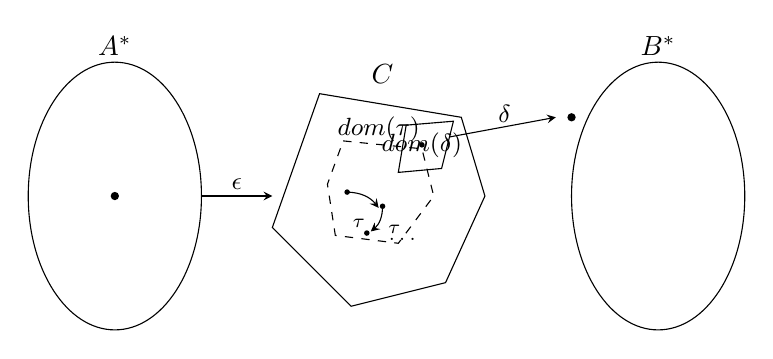
\begin{tikzpicture}[>=stealth, scale=1]

% A*
\draw (0,0) ellipse (1.1cm and 1.7cm);
\node at (0,1.9) {$A^*$};
\fill (0,0) circle (1.5pt);

% C (poligono irregolare)
\draw (2.6,1.3) -- (4.4,1.0) -- (4.7,0) -- (4.2,-1.1) -- (3.0,-1.4) -- (2.0,-0.4) -- cycle;
\node at (3.4,1.55) {$C$};

% dom(tau), regione tratteggiata dentro C
\draw[dashed] (2.9,0.7) -- (3.9,0.6) -- (4.05,0) -- (3.6,-0.6) -- (2.8,-0.5) -- (2.7,0.15) -- cycle;
\node[font=\small] at (3.35,0.85) {$dom(\tau)$};

% punti e frecce tau (successione di transizioni)
\fill (2.95,0.05) circle (1pt);
\draw[->] (2.95,0.05) to[bend left=25] (3.35,-0.15);
\node[font=\scriptsize] at (3.1,-0.35) {$\tau$};

\fill (3.4,-0.13) circle (1pt);
\draw[->] (3.4,-0.13) to[bend left=25] (3.25,-0.45);
\node[font=\scriptsize] at (3.55,-0.42) {$\tau$};

\fill (3.2,-0.47) circle (1pt);
\node[font=\scriptsize] at (3.65,-0.55) {$\ldots$};

% dom(delta)
\draw (3.7,0.9) -- (4.3,0.95) -- (4.15,0.35) -- (3.6,0.3) -- cycle;
\node[font=\small] at (3.9,0.65) {$dom(\delta)$};
\fill (3.9,0.65) circle (1pt);

% freccia epsilon: A* -> C
\draw[->] (1.1,0) -- (2.0,0);
\node[font=\small] at (1.55,0.15) {$\epsilon$};

% freccia delta: dom(delta) -> B*
\draw[->] (4.25,0.75) -- (5.6,1.0);
\node[font=\small] at (4.95,1.05) {$\delta$};
\fill (5.8,1.0) circle (1.5pt);

% B*
\draw (6.9,0) ellipse (1.1cm and 1.7cm);
\node at (6.9,1.9) {$B^*$};

\end{tikzpicture}
\end{center}

\footnotetext{Tesi di Church: l'insieme dei risultati di equivalenza tra vari modelli effettivi di calcolo è noto come Tesi di Church, che afferma che tutti i modelli di calcolo si equivalgono.}

\begin{defi}[Funzione associata ad un algoritmo]Sia $\mathcal A:=(A,B,C,\epsilon, \tau, \delta)$ un algoritmo. Possiamo definire la funzione
\[
\begin{matrix}
f_\mathcal{A} : & A^* & \to & B^*
\\
& w & \mapsto &  \begin{cases} \delta(\tau^n(\epsilon(w))) & \text{se } n \text{ è il più piccolo intero}
\\ & \text{per cui } \tau^n(\epsilon(w)) \in dom(\delta) \text{ ,} 
\\ \bot & \text{se } \mathcal A \text{ non termina partendo da } w \end{cases}
\end{matrix}
\]
che chiameremo \textit{funzione associata all'algoritmo} $\mathcal A$.
\end{defi}

In pratica, ogni volta che diremo che la funzione $f$ associata ad un certo algoritmo formale è definita per ogni possibile parola $w \in A^*$, intenderemo dire che per ogni possibile input la computazione termina e restituisce attraverso la funzione di output $\delta$ il valore della funzione $f(w)$.

\begin{defi}[Funzione caratteristica]
La funzione $\mathbf{1}_X$ è la \textit{funzione caratteristica} (o indicatrice) dell'insieme $X$, definita come
\[
\mathbf{1}_X(w) = \begin{cases} 1 & w \in X \\ 0 & w \notin X. \end{cases}
\]
\end{defi}

\begin{defi}[Algoritmo che decide un insieme]
Diremo che un certo \textit{algoritmo decide} un insieme $X \subset A^*$ quando la funzione associata all'algoritmo coincide con la funzione caratteristica di $X$, quindi se vale:
\[
f_\mathcal{A}(x) = \mathbf{1}_X(x) \text{ per ogni } x \in A^*.
\]
\end{defi}
\begin{defi}[Algoritmo che semidecide un insieme]
Diremo che un certo algoritmo  \textit{semidecide} un insieme
$X \subseteq A^*$ quando la funzione parziale associata all'algoritmo
$f_{\mathcal A}$ è definita esattamente sugli elementi di $X$ e, quando è
definita, restituisce il valore $1$. In altre parole:
\[
f_{\mathcal A}(x)=
\begin{cases}
1, & \text{se } x\in X,\\
\bot, & \text{se } x\notin X,
\end{cases}
\]
dove il simbolo $\bot$ indica che l'algoritmo non termina.
\end{defi}

\begin{rema}
Questa è chiaramente una funzione totale pertanto nella definizione, implicitamente, stiamo affermando che quando un algoritmo decide un insieme, la computazione dell'algoritmo a partire da una qualsiasi parola di alfabeto $A$ termina.
\end{rema}
\textcolor{red}{controlla qui:}
Pertanto, consideriamo i processi computazionali come metodi di decisione simbolici, in cui si rende automatico (per questo formalmente ineccepibile) il metodo di decisione di una proprietà. Le garanzie sulla correttezza della decisione vengono dalla verificabilità: il processo lavora su sequenze di simboli, e applica in maniera asettica alcune regole di trasformazione (i principi deduttivi) in maniera puntuale: da cui viene la richiesta specifica che le regole di trasformazione siano locali, applicabili in tempo finito e soprattutto in modo che la verifica della corretta applicazione sia finita.

In questo quadro, se anche il problema di decisione riguardasse un insieme di cardinalità più che numerabile, un processo computazionale finito potrebbe procedere modificando ed essendo influenzato solo da un numero finito di elementi. Quindi è la descrizione stessa del problema che ha senso solo quando è finita.

Con queste premesse la classe dei problemi più semplici che si possono porre è in prima istanza quella dei \textit{problemi di decisione} per un fissato alfabeto $A = \{a_1, \dots, a_n\}$. Essi consistono nella possibilità di definire un metodo per stabilire la separazione tra le parole di un sottoinsieme $X \subset A^*$ e quelle del complemento $A^* \setminus X$, procedura con le caratteristiche che abbiamo ricordato.

\newpage

\section{Automi a stati finiti}
\subsection{Definizione di automa a stati finiti.}

\begin{defi}\label{def:1}
Siano $A$ e $Q$ insiemi finiti, un \textit{automa finito} di alfabeto $A$ e insieme degli stati $Q$  è una tripla $(T,q_0,F)$ dove
\[
T: Q\times A \to Q
\]
$F \subset Q$ e $q_0\in Q$ è uno stato particolare, detto stato iniziale.
\end{defi}


\subsection{Definizione di algoritmo associato ad un automa}

A partire dalla tripla $(T,q_0,F)$ che specifica un dato automa di alfabeto $A$ e insieme degli stati $Q$ si costruisce prima l'insieme delle configurazioni possibili:

\begin{defi}[Configurazione per Automa Finito]\label{def:3}
Una configurazione per automa a stati finiti di alfabeto $A$ e insieme degli stati $Q$ è una tripla $(w,p,q)$, dove
\begin{enumerate}
    \item $w\in A^*$ è la parola da analizzare,
    \item $p\in\mathbb{N}$, è un intero che indica la posizione della parola da analizzare nella prossima transizione,
    \item $q\in Q$ indica lo stato corrente e costituisce la memoria delle transizioni effettuate nei precedenti passi di computazione.
\end{enumerate}
\end{defi}

L'insieme delle configurazioni di alfabeto $A$ e insieme degli stati $Q$ per automa finito sarà denotato con
\[
Conf_{DFA}^{A,Q} = A^* \times \mathbb{N} \times Q
\]
ed allora possiamo definire:

\begin{defi}[Algoritmo associato ad un automa finito deterministico]\label{def:4}
L'algoritmo associato ad un automa di alfabeto $A$ e insieme degli stati $Q$ è l'algoritmo $$(A,Conf_{DFA}^{A,Q}, \{0,1\},\epsilon,\tau,\delta)$$ dove le tre funzioni sono definite come segue:
\begin{itemize}
    \item la \textbf{funzione di ingresso} che associa ad una parola $w\in A^*$, la configurazione $\varepsilon(w) = (w,1,q_0)$,

    \item la \textbf{funzione di transizione} $\tau: Conf_{DFA}^{A,Q} \to Conf_{DFA}^{A,Q}$ è data da
    \[
    \tau((w,p,q)) = (w,p+1,T(q,w(p))),
    \]

    \item la \textbf{funzione di uscita} $\delta: Conf_{DFA}^{A,Q} \to \{0,1\}*$, data da
    \[
    \delta((w,p,q)) =
    \begin{cases}
    0 & \text{se } p>|w| \text{ e se } q\notin F, \\
    1 & \text{se } p>|w| \text{ e se } q\in F.
    \end{cases}
    \]
\end{itemize}
\end{defi}



\begin{defi}[Insiemi decidibili per automa]\label{def:5}
Un insieme $X\subset A^*$, è \textit{decidibile} per automa finito (oppure \textit{DFA-decidibile} oppure \textit{regolare}), se esiste un insieme finito $Q$ e un automa finito con alfabeto $A$ e insieme degli stati $Q$ tale che l'algoritmo associato decide $X$.
\end{defi}
\begin{exam}\label{ex: parole lunghezze pari}
Descrivere l'automa finito che decide l'insieme delle parole di lunghezza pari (risp. dispari) su un alfabeto dato $A$.

A partire dall'alfabeto finito $A$, e da un insieme di due stati $Q=\{0,1\}$ che corrisponderanno rispettivamente allo stato ``abbiamo letto un numero pari (oppure dispari) di caratteri della parola''; costruiamo la funzione di transizione che ad ogni carattere letto cambia stato:
\[
T: Q\times A \to Q
\]
tale che
\[
T(q,a) =
\begin{cases}
1 & \text{se } q=0 \\
0 & \text{se } q=1,
\end{cases}
\]
per ogni $a\in A$.

Avremo allora che lo stato iniziale $q_0=0$, poiché inizialmente non avremo ancora letto nessun carattere e che l'insieme degli stati accettanti sarà: $F=\{0\}$.
\begin{proof}
Sia
\[
X=\{\,w\in A^* : |w|\text{ è pari}\,\}.
\]
Dimostriamo che l'algoritmo associato all'automa
\[
(T,q_0,F)
\]
decide l'insieme \(X\).

Sia dunque \(w=a_1a_2\cdots a_n\in A^*\). La configurazione iniziale è
\[
\epsilon(w)=(w,1,0).
\]

Ad ogni applicazione della funzione di transizione viene letta una lettera della parola e lo stato viene invertito:
\[
0\longleftrightarrow1.
\]
Per induzione sul numero di transizioni effettuate si ottiene che dopo aver letto i primi \(k\) caratteri della parola la configurazione è
\[
(w,k+1,q_k),
\]
dove
\[
q_k=
\begin{cases}
0 & \text{se } k \text{ è pari},\\
1 & \text{se } k \text{ è dispari}.
\end{cases}
\]

Dopo la lettura dell'intera parola si raggiunge quindi la configurazione
\[
(w,n+1,q_n).
\]
Poiché
\[
n+1>|w|,
\]
questa appartiene al dominio della funzione di uscita. Inoltre
\[
q_n=
\begin{cases}
0 & \text{se } |w| \text{ è pari},\\
1 & \text{se } |w| \text{ è dispari}.
\end{cases}
\]

Essendo \(F=\{0\}\), segue che
\[
\delta(w,n+1,q_n)=
\begin{cases}
1 & \text{se } |w| \text{ è pari},\\
0 & \text{se } |w| \text{ è dispari}.
\end{cases}
\]

Pertanto
\[
f_{\mathcal A}(w)=
\begin{cases}
1 & \text{se } w\in X,\\
0 & \text{se } w\notin X,
\end{cases}
\]
cioè
\[
f_{\mathcal A}=\mathbf 1_X.
\]

Ne consegue che l'algoritmo associato all'automa decide l'insieme delle parole di lunghezza pari.
\end{proof}
\end{exam}
\begin{ex}\label{es:1}
Fissiamo l'alfabeto binario $A=\{0,1\}$, dimostrare che l'insieme
\[
X = \{ w0 \mid w\in A^* \}
\]
è decidibile per automa a stati finiti.


\textbf{Soluzione.} Si richiede di mostrare un automa il cui algoritmo associato accetta le parole che terminano con uno zero. È dunque sufficiente memorizzare nello stato l'ultimo simbolo letto e alla fine della lettura della parola decidere in base allo stato: poniamo $Q=\{q_0,q_1\}$, e definiamo
\[
T(q,a) :=
\begin{cases}
q_0 & \text{se } a=0, \\
q_1 & \text{se } a=1,
\end{cases}
\]
prendiamo $q_0$ come stato iniziale e $F=\{q_0\}$ come insieme degli stati finali accettanti.
\end{ex}
\begin{proof}
Sia
\[
X=\{w0\mid w\in A^*\}
\]
l'insieme delle parole sull'alfabeto binario che terminano con il simbolo \(0\).

Costruiamo un automa finito che decide \(X\). Consideriamo l'insieme degli stati
\[
Q=\{q_0,q_1\},
\]
dove intuitivamente:
\begin{itemize}
    \item \(q_0\) rappresenta la situazione in cui l'ultimo simbolo letto è \(0\);
    \item \(q_1\) rappresenta la situazione in cui l'ultimo simbolo letto è \(1\).
\end{itemize}

Definiamo la funzione di transizione
\[
T:Q\times A\to Q
\]
come
\[
T(q,a)=
\begin{cases}
q_0 & \text{se } a=0,\\
q_1 & \text{se } a=1.
\end{cases}
\]

Scegliamo come stato iniziale
\[
q_{\mathrm{init}}=q_0
\]
e come insieme degli stati accettanti
\[
F=\{q_0\}.
\]

Consideriamo ora l'algoritmo associato all'automa.
Sia
\[
w=a_1a_2\cdots a_n\in A^*.
\]
La configurazione iniziale è
\[
\epsilon(w)=(w,1,q_0).
\]

Dopo \(k\) transizioni, per induzione su \(k\), la configurazione raggiunta è
\[
(w,k+1,q_k),
\]
dove
\[
q_k=
\begin{cases}
q_0 & \text{se } a_k=0,\\
q_1 & \text{se } a_k=1.
\end{cases}
\]

Infatti, ad ogni passo la funzione di transizione sostituisce lo stato corrente con lo stato corrispondente all'ultimo carattere letto.

Dopo aver letto tutta la parola \(w\), la computazione termina nella configurazione
\[
(w,n+1,q_n).
\]
La funzione di uscita restituisce quindi
\[
\delta(w,n+1,q_n)=
\begin{cases}
1 & \text{se } q_n\in F,\\
0 & \text{se } q_n\notin F.
\end{cases}
\]

Poiché
\[
F=\{q_0\},
\]
si ha
\[
\delta(w,n+1,q_n)=
\begin{cases}
1 & \text{se l'ultimo simbolo di } w \text{ è }0,\\
0 & \text{se l'ultimo simbolo di } w \text{ è }1.
\end{cases}
\]

Quindi
\[
f_{\mathcal A}(w)=
\begin{cases}
1 & \text{se } w\in X,\\
0 & \text{se } w\notin X.
\end{cases}
\]

Pertanto
\[
f_{\mathcal A}=\mathbf 1_X
\]
e quindi l'algoritmo associato all'automa decide \(X\).

Concludiamo che
\[
X=\{w0\mid w\in A^*\}
\]
è DFA-decidibile.
\end{proof}

\newpage


\section{Rappresentazione grafica degli automi}
\subsection{Automi come grafi}
A partire da un automa finito $(T,q_0,F)$ se ne può dare una descrizione grafica nel modo seguente: si consideri il grafo i cui nodi sono gli stati $Q$, e gli archi etichettati con elementi di $A$ che collegano due stati $(q_i,q_j)$ se esiste la transizione $T(q_i,a)=q_j$.
inoltre avremo una funzione che ci indica lo stato iniziale
\[
\texttt{init}(G_{(T,q_0,F)}) = q_0
\]
(di solito indicata da un arco entrante nel nodo iniziale $q_0$) ed una che distingue gli stati accettanti (risp. non accettanti)
\[
\texttt{acc}(G_{(T,q_0,F)}) = F \qquad (\text{risp. } \texttt{ref}(G_{(T,q_0,F)}) = Q \setminus F)
\]
(di solito si indicano gli stati accettanti con un doppio cerchio, mentre tutti gli altri nodi sono considerati non accettanti).
Per essere più formali:
\begin{defi}[Grafo associato ad un automa]
Dato un automa $(T,q_0,F)$ definito su un alafabeto $A$ e insieme di stati $Q$ definiamo il suo grafo associato $G=(V,E,L)$ come segue:
\begin{itemize}
    \item l'insieme dei vertici è
    \[
    V:=Q;
    \]
    \item l'insieme dei lati è
    \[
    E:=\{(q_i,a,q_j)\in Q\times A\times Q \mid T(q_i,a)=q_j\};
    \]
    \item la funzione di etichettatura è
    \[
    L:E\to A, \qquad L(q_i,a,q_j)=a.
    \]
\end{itemize}
\end{defi}

Ad esempio il grafo associato all'automa dell'Esempio~\ref{ex: parole lunghezze pari}, è rappresentato in Figura~\ref{figura esempio automa per parole pari}.
\begin{figure}[ht]
\centering
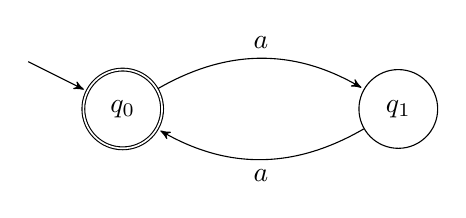
\begin{tikzpicture}[
    ->, >=stealth', shorten >=1pt, auto, node distance=3.5cm,
    every state/.style={circle, draw, minimum size=1cm}
]
    \node[state, accepting] (q0) {$q_0$};
    \node[state] (q1) [right of=q0] {$q_1$};

    \draw[->] (-1.2,0.6) -- (q0);
    \path (q0) edge [bend left=30] node {$a$} (q1)
          (q1) edge [bend left=30] node {$a$} (q0);
\end{tikzpicture}
\caption{Automa dell'Esempio \ref{ex: parole lunghezze pari}, notare che $a$ è un qualsiasi elemento nell'alfabeto $A=\{0,1\}$.}
\label{figura esempio automa per parole pari}
\end{figure}
\begin{figure}[h]
\centering
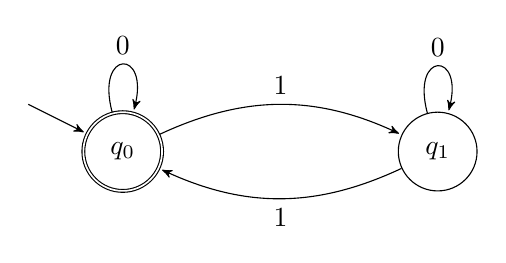
\begin{tikzpicture}[
    ->, >=stealth', shorten >=1pt, auto, node distance=4cm,
    every state/.style={circle, draw, minimum size=1cm}
]
    \node[state, accepting] (q0) {$q_0$};
    \node[state] (q1) [right of=q0] {$q_1$};

    \draw[->] (-1.2,0.6) -- (q0);

    \path (q0) edge [loop above] node {$0$} (q0)
          (q1) edge [loop above] node {$0$} (q1)
          (q0) edge [bend left=25] node {$1$} (q1)
          (q1) edge [bend left=25] node {$1$} (q0);
\end{tikzpicture}
\caption{In modo simile all'automa dell'Esempio~\ref{ex: parole lunghezze pari} si può dare l'automa che decide l'insieme di tutte le parole con un numero pari di 1.}
\label{fig:parita}
\end{figure}

% =========================================================
% FIGURA 3
% =========================================================
\begin{figure}[ht]
\centering
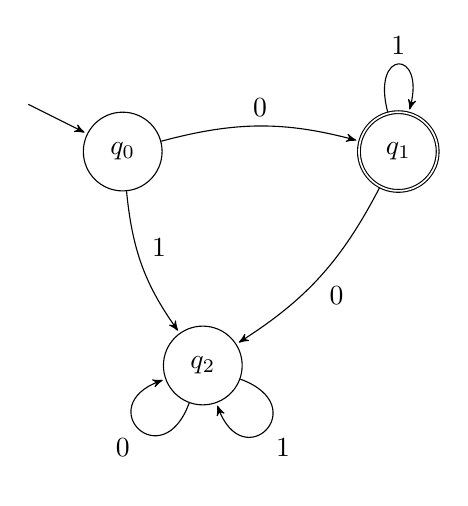
\begin{tikzpicture}[
    ->, >=stealth', shorten >=1pt, auto, node distance=3.5cm,
    every state/.style={circle, draw, minimum size=1cm}
]
    \node[state] (q0) {$q_0$};
    \node[state, accepting] (q1) [right of=q0] {$q_1$};
    \node[state] (q2) [below right=2cm and 0.3cm of q0] {$q_2$};

    \draw[->] (-1.2,0.6) -- (q0);

    \path (q0) edge [bend left=15] node {$0$} (q1)
          (q1) edge [loop above] node {$1$} (q1)
          (q0) edge [bend right=15] node {$1$} (q2)
          (q1) edge [bend left=15] node {$0$} (q2)
          (q2) edge [loop below, min distance=10mm, in=200, out=250] node[below left] {$0$} (q2)
          (q2) edge [loop below, min distance=10mm, in=290, out=340] node[below right] {$1$} (q2);
\end{tikzpicture}
\caption{Automa che decide l'insieme $X=\{01^n \mid n\geq 0\}$.}
\label{fig:01n}
\end{figure}

\begin{comment}
\subsection{Rappresentazione come matrice di adiacenza}

Possiamo usare $M_E$ per indicare la matrice di adiacenza del grafo $G=(V,E)$ definita come 
\[
(M_E)_{ij} =
\begin{cases}
1 & \text{se } (v_i,v_j) \in E \\
0 & \text{altrimenti.}
\end{cases}
\]
Ad esempio, in Figura~\ref{fig:grafo7}, abbiamo un grafo orientato e la corrispondente matrice di adiacenza.
È sensato, che ad ogni insieme $E$ corrisponda un'unica matrice una volta che è fissato un ordinamento degli elementi di $V$. Utilizzando le  operazioni aritmetiche  date dal semianello dei booleani $(\mathbb{B}, \vee, \wedge)$:

\[
\mathbb{B} = \{0,1\} \qquad
\begin{array}{c|cc}
a \vee b & a & b \\
\hline
0 & 0 & 0 \\
1 & 1 & 0 \\
1 & 0 & 1 \\
1 & 1 & 1
\end{array}
\qquad
\begin{array}{c|cc}
a \wedge b & a & b \\
\hline
0 & 0 & 0 \\
0 & 1 & 0 \\
0 & 0 & 1 \\
1 & 1 & 1
\end{array}
\]
possiamo definire il prodotto seguente
\[
A=(a_{ij})\in\mathbb{B}^{m\times n},
\qquad
B=(b_{ij})\in\mathbb{B}^{n\times p},
\]
\[
(AB)_{ij}
:=
\bigvee_{k=1}^{n}
\left(a_{ik}\wedge b_{kj}\right),
\qquad
1\le i\le m,\;1\le j\le p.
\]
Usando il prodotto definito sopra,
la matrice $M_E^2$ ha un 1 in posizione $i,j$ se esiste un cammino di lunghezza esattamente 2 che va dal vertice $v_i$ al vertice $v_j$, questo equivale a dire che esiste (almeno) un vertice $w$ tale che $(v_i,w),(w,v_j) \in E$.
Inoltre, si può provare per induzione su $k$ il seguente fatto:
\begin{prop}
       $(M_E^k)_{ij}=1$ se e solo se esiste un cammino di lunghezza esattamente $k$ da $v_i$ a $v_j$.
\end{prop}

\begin{rema}\textcolor{red}{controlla}
 La chiusura riflessiva e transitiva di $G$ si può ottenere come limite delle somme parziali delle potenze successive di $M_E^k$:
\[
M_E^* = \sum_{i\geq 0} M_E^i
\]

Si noti come in questo caso la somma infinita può essere limitata da un intero $L$ che certamente esiste e che corrisponde alla massima lunghezza del cammino più breve che connette una coppia di nodi (per ogni coppia). Una volta calcolata la potenza corrispondente a tale lunghezza, il valore della somma non sarà modificata ulteriormente:
\[
M_E^* = \sum_{i=0}^{L} M_E^i.
\]
\end{rema}

\end{comment}

\subsection{Matrici di adiacenza per grafi di automi finiti}
Consideriamo un automa 
$(T,q_0,F)$ definito su un alafabeto 
$A$ e insieme di stati $Q$.
Possiamo sempre considerare il monoide $M=(A^*,A^\emptyset, \cdot)$ 
e l'anello (che e/' anche un semianello) $\mathbb N$.
A questo punto possiamo definire l'insieme delle serie formali
\[
\mathbb N [M]
:=
\left\{
    \sum_{w \in A^*}n_w w \, | \, n_w \in \mathbb N 
\right\}
\]
Ora possiamo considerare la matrice di adiacenza $Z$ dell'automa,
che non sarà nient'altro che una matrice cha nelle entrate elementi di $\mathbb N[M]$.
Come sappiamo, fare la potenza $k$-esima di una matrice di adiacenza con etichette,
fornisce nell'entrata $(i,j)$
tutti e i soli cammini di lunghezza $k$ che collegano il vertice
$i$ al vertice $j$ (nel caso degli automi, dallo stato $q_i$ allo stato $q_j$).
Vediamo un esempio:
\begin{exam}
    Consideriamo l'automa che decide l'inisieme delle parole di lunghezza pari. 
    Questo e/' rappresentato dal seguente grafo etichettato.
\begin{center}
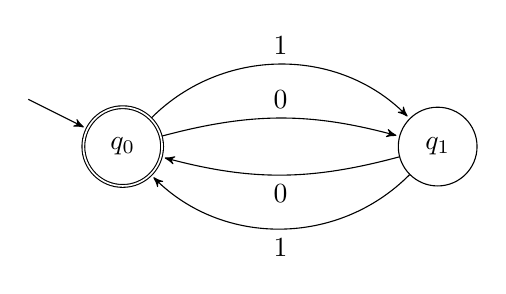
\begin{tikzpicture}[
    ->, >=stealth', shorten >=1pt, auto, node distance=4cm,
    every state/.style={circle, draw, minimum size=1cm}
]
    % Stati (q0 ha il doppio cerchio con 'accepting')
    \node[state, accepting] (even) {$q_0$};
    \node[state] (odd) [right of=even] {$q_1$};

    % Freccia iniziale esterna
    \draw[->] (-1.2,0.6) -- (even);

    % Transizioni SOPRA (da q0 a q1)
    \path (even) edge [bend left=45] node[above] {$1$} (odd);
    \path (even) edge [bend left=15] node[above] {$0$} (odd);

    % Transizioni SOTTO (da q1 a q0)
    \path (odd) edge [bend left=45] node[below] {$1$} (even);
    \path (odd) edge [bend left=15] node[below] {$0$} (even);
\end{tikzpicture}
\end{center}
La sua matrice di adiacenza e/'
\[
Z=
\begin{pmatrix}
   \bot & 0 + 1
    \\
    0+1 & \bot
\end{pmatrix}
\]
Infatti, gli archi $0$ e $1$ collegano i vertici 
$q_0$ e $q_1$ in entrambe le direzioni.
Inoltre, visto che non ci sono loop, 
sulla diagonale si inserisce convenzionalmente la serie formale vuota, 
indicata con $\bot$.
A questo punto vogliamo trovare i cammini di lunghezza 2 del grafo.
Per farlo basta calcolare la potenza seconda di $Z$:
\begin{align*}
Z^2&=
\begin{pmatrix}
    \bot \bot + (0+1)(0+1) & \bot(0+1) + (0+1)\bot
    \\[6pt]
    (0+1)\bot + \bot(0+1) & (0+1)(0+1) + \bot \bot
\end{pmatrix}
\\ &=
\begin{pmatrix}
    00+ 01+ 10+11 & \bot + \bot
    \\[6pt]
    \bot + \bot &  00+ 01+ 10+11
\end{pmatrix}
\\ &=
\begin{pmatrix}
    00+ 01+ 10+11 &  \bot
    \\[6pt]
    \bot &  00+ 01+ 10+11
\end{pmatrix}
\end{align*}
Per verificare le operazioni effettuate con $\bot$, 
basta usare la definizione presente in (\ref{def:serie-formali}).
Dalla matrice possiamo quindi dedurre che
esistono 4 cammini che collegano $q_0$ e $q_1$ con loro stessi,
e nessuno che collega $q_0$ con $q_1$ o viceversa.
\end{exam}

A questo punto ci vogliamo porre la seguente domanda: 
si può dedurre dala matrice di adiacenza tutti i cammini che uniscono lo stato iniziale
ad uno stato accettante dell'automa?
In altre parole:
dalla matrice di adiacenza si può dedurre il calcolo che l'automa compie per decidere un insieme?
La risposta e' si.
In partiolare, e/' anche possibile dedurre l'intero insieme $X$ da decidere.
Prima di affrontare il caso generale
analizziamo questo problema nel caso dell'esempio precedente.
\begin{exam}
    In questo caso esiste un solo stato accettante,
    che coincide esattamente con lo stato iniziale.
    Quindi,
    in una qualsiasi potenza di $Z$,
    dovremmo considerare l'entrata $(1,1)$
    per trovare le parole accettate dall'automa.
    Più precisamente, per ogni $k$ naturale, nell'entrata $(1,1)$
    della matrice $Z^k$
    troviamo le uniche e sole parole
    di lunghezza $k$ accettate dall'automa.
\end{exam}
Lavoriamo ora al caso generale. Se con $Z$ indichiamo la matrice di adiacenza di un automa,
possiamo definire
definiamo
\[
E(Z)
:=
\sum_{k=0}^\infty Z^k
\]
dove $Z^0$ e/' la matrice cha ha sulla diagonale la parola vuota $A^\emptyset$
e nelle altre entrate la serie vuota $\bot$.
Assumendo che lo stato iniziale sia $q_0$
e che corrisponda alla prima riga della matrice $Z$,
allora sulla prima riga di $E(Z)$
troveremo le parole che l'automa accetta nelle colonne corrispondenti
agli stati accettanti.
\begin{exam}
    Facendo ancora un paio di potenze di $Z$, 
    si può dedurre la seguente formula:
    \[
    Z^k=
    \left\{
    \begin{matrix}
        \begin{pmatrix}
            (0+1)^k & \bot
            \\
            \bot & (0+1)^k
        \end{pmatrix}
        ,& \text{se } k \text{ e/' pari}
        \\
        \\
        \begin{pmatrix}
            \bot & (0+1)^k
            \\
            (0+1)^k & \bot
        \end{pmatrix}
        ,& \text{se } k \text{ e/' dispari}
    \end{matrix}
    \right.
    \]
    quindi abbiamo
    \begin{align*}
    E(Z)&=
    \begin{pmatrix}
        A^\emptyset & \bot
        \\
        \bot & A^\emptyset
    \end{pmatrix}
    +
    \begin{pmatrix}
            \bot & (0+1)
            \\
            (0+1) & \bot
    \end{pmatrix}
    +
    \begin{pmatrix}
            (0+1)^2 & \bot
            \\
            \bot & (0+1)^2
        \end{pmatrix}
    + \cdots
    \\&=
    \begin{pmatrix}
        A^\emptyset + \sum_{k =1}^{\infty}(0+1)^{2k} & \bot + \sum_{k =0}^{\infty}(0+1)^{2k+1}
        \\
        \bot + \sum_{k =0}^{\infty}(0+1)^{2k+1} &  A^\emptyset + \sum_{k =1}^{\infty}(0+1)^{2k} 
    \end{pmatrix}
    \\&=
    \begin{pmatrix}
        A^\emptyset + \sum_{k =1}^{\infty}(0+1)^{2k} & \sum_{k =0}^{\infty}(0+1)^{2k+1}
        \\
        \sum_{k =0}^{\infty}(0+1)^{2k+1} &  A^\emptyset + \sum_{k =1}^{\infty}(0+1)^{2k} 
    \end{pmatrix}
    \end{align*}
    Per quanto osservato prima,
    nel posto $(1,1)$ della matrice
    $E(Z)$ troviamo le uniche e solo parole accettate dall'automa.
    \textcolor{red}{Non coverrebbe scrivre E(Z) a partire con k=1? perhce ha priori non e/' vero che la parola vuota e/' decidibile}
\end{exam}
Usando un po' di algebra lineare,
e/' possibile esplicitare esattamente l'inisieme delle parole accettate.
Infatti, fi possiamo definire i seguenti vettori:
\[
V_0(i)=
\left\{
\begin{matrix}
    A^\emptyset,  & q_i=q_0 
    \\
    \bot, & q_i\neq q_0 
\end{matrix}
\right.
\]
\[
V_F(i)=
\left\{
\begin{matrix}
    A^\emptyset,  & q_i \in F
    \\
    \bot, & q_i\notin F
\end{matrix}
\right.
\]
E calcolando il prodotto righe per colonne
\[
V_0 \cdot E(Z) \cdot V_F^t
\]
otteniamo la serie formale che ha come addendi esattamente le parole accettate da $X$.
La formula appena enunciata prende il nome di \textit{formula dell'esecuzione}.
\footnote{Ricordiamo che $\bot$ e/' l'elemento neutro additivo, 
che $A^\emptyset$ e/' l'elemento neutro moltiplicativo,
e che $\bot \cdot w = \bot$ per ogni serie formale $w \in \mathbb N[M]$.
}
\begin{exam}
    Nel caso dell'esempio precedente abbiamo
    \[
    V_0=(A^\emptyset, \bot)
    \]
    \[
    V_F=(A^\emptyset, \bot)
    \]
    Facendo il prodotto abbiamo
    \begin{align*}
        V_0 \cdot E(Z) \cdot V_F^t
        &=
        \begin{pmatrix}
              A^\emptyset & \bot    
        \end{pmatrix}
        \cdot 
        \begin{pmatrix}
        A^\emptyset + \sum_{k =1}^{\infty}(0+1)^{2k} & \sum_{k =0}^{\infty}(0+1)^{2k+1}
        \\
        \sum_{k =0}^{\infty}(0+1)^{2k+1} &  A^\emptyset + \sum_{k =1}^{\infty}(0+1)^{2k} 
    \end{pmatrix}
        \cdot
        \begin{pmatrix}
            A^\emptyset
            \\
            \bot
        \end{pmatrix}
        \\
        &=
        \begin{pmatrix}
            A^\emptyset + \sum_{k =1}^{\infty}(0+1)^{2k}
            &
            \sum_{k =0}^{\infty}(0+1)^{2k+1}
        \end{pmatrix}
        \cdot
        \begin{pmatrix}
            A^\emptyset
            \\
            \bot
        \end{pmatrix}
        \\&=
         A^\emptyset + \sum_{k =1}^{\infty}(0+1)^{2k}
    \end{align*}
    Che e/' esattamente quanto abbiamo osservato precedentemente.
\end{exam}

\newpage


\section{Linguaggi regolari}
Per determinare se un determinato linguaggio è regolare: mentre la dimostrazione sufficiente di AF-
decidibilità (esibendo esplicitamente un automa) può risultare noiosa e complicata, è possibile fornire dimo-
strazioni alternative (possibilmente più semplici) mostrando che l’insieme è ottenibile a partire da insiemi
AF-decidibili utilizzando operazioni “compatibili” con l’AF-decidibilità (proprietà di chiusura).
In questa sezione vedremo dunque che esistono operazioni fatte su insiemi AF-decidibili che permettono
di ottenere un altro insieme DFA-decidibile.
\begin{defi}
    Sia $A$ un alfabeto e $X_1$ e $x_2$ due inisemi di parole su $A$, ovvero $X_1,X_2 \subset A^*$. Definiamo allora:
    \begin{itemize}
    \item l'operazione di \emph{concatenazione}:
    \[
    X_1 \cdot X_2 := \{ w_1 w_2 \in A^* \mid w_i \in X_i \};
    \]

    \item l'operazione di \emph{somma}:
    \[
    X_1 + X_2 := \{ w \in A^* \mid w \in X_1 \text{ oppure } w \in X_2 \}
    \]
    (di fatto, è l'unione insiemistica di $X_1$ con $X_2$);

    \item l'operazione di \emph{star di Kleene}:
    \[
    X^* := \{ w_1 w_2 \dots w_n \mid w_i \in X, \text{for } i=1,\dots,n \text{ e } n\geq 0 \}
    \]
\end{itemize}

\end{defi}

\begin{prop}\label{prop:8}
Siano $X_1$ e $X_2$ regolari allora anche $X_1+X_2$ è regolare.


\begin{proof}
    
Sia $\mathcal{A}_1 = (T_1,q_0,F_1)$ l'automa che decide l'insieme $X_1$ e sia $\mathcal{A}_2 = (T_2,q_0',F_2)$ l'automa che decide $X_2$.
L'automa che riconosce $X_1+X_2$ è ottenuto utilizzando il prodotto cartesiano degli stati dei due automi e calcolando l'evoluzione ``parallela'' di entrambi gli automi a partire da uno stato coppia, in questo modo se una delle due componenti dello stato è accettante alla fine della computazione la parola sarà accettata poiché apparterrà ad uno dei due insiemi e quindi sarà nella loro unione.

Costruzione dell'automa $\mathcal{A} = (T,q_0'',F)$ di alfabeto $A$ e insieme degli stati $Q = Q_1\times Q_2$: definiamo
\[
q_0'' = (q_0,q_0'), \qquad F = F_1\times Q_2 \cup Q_1\times F_2
\]

e
\[
T((q_1,q_2),a) = (T_1(q_1,a), T_2(q_2,a)).
\]
Mostriamo che $\mathcal{A}$ decide precisamente $X_1+X_2$.
\[
T^*((q_0,q_0'),w)
=
\left(T_1^*(q_0,w),T_2^*(q_0',w)\right).
\]

Mostriamo ora che l'automa $\mathcal{A}$ decide l'insieme $X_1+X_2$, 
ovvero che la funzione associata all'automa coincide con la funzione caratteristica
di tale insieme.

Sia $w\in A^*$. Dalla definizione dell'insieme degli stati finali si ha:
\[
\begin{aligned}
f_{\mathcal{A}}(w)=1
&\iff
T^*((q_0,q_0'),w)\in F\\
&\iff
\left(T_1^*(q_0,w),T_2^*(q_0',w)\right)
\in (F_1\times Q_2)\cup(Q_1\times F_2)\\
&\iff
T_1^*(q_0,w)\in F_1
\ \text{oppure}\
T_2^*(q_0',w)\in F_2\\
&\iff
f_{\mathcal{A}_1}(w)=1
\ \text{oppure}\
f_{\mathcal{A}_2}(w)=1\\
&\iff
w\in X_1
\ \text{oppure}\
w\in X_2\\
&\iff
w\in X_1+X_2.
\end{aligned}
\]

Quindi, per ogni $w\in A^*$,
\[
f_{\mathcal{A}}(w)=\mathbf{1}_{X_1+X_2}(w).
\]

Pertanto l'automa $\mathcal{A}$ decide l'insieme $X_1+X_2$, e quindi
$X_1+X_2$ è regolare.
\end{proof}
\end{prop}


\begin{ex}\label{es:3}
Si consideri l'alfabeto $A=\{0,1\}$ e sia $B=\{1\}$ la restrizione all'insieme che contiene il solo simbolo $1$; si considerino l'insieme delle parole di alfabeto $A$ di lunghezza pari:
\[
X_1 = \{ w \in A^* \mid |w| = 2n,\ n\geq 0 \}
\]
e l'insieme delle parole di alfabeto $A$ che contengono un numero pari di $1$:
\[
X_2 = \{ w \in A^* \mid |w_{|B}| = 2k,\ k\geq 0 \}
\]
qui si è utilizzata la notazione $w_{|B}$ per indicare la parola $w$ ristretta ai soli elementi di alfabeto $B$, (si noti che si tratta degli insiemi considerati in Figura~\ref{fig:automa} e in Figura~\ref{fig:parita}).

Costruire l'automa che decide $X_1+X_2$.


\begin{proof}
L'automa si può ottenere utilizzando la costruzione di composizione parallela utilizzata nella prova della proposizione a partire dai due automi per $X_1$ e $X_2$.
\end{proof}
\end{ex}


Mostriamo ora un'altra proprietà di chiusura degli insiemi regolari: la classe degli insiemi regolari è chiusa per concatenazione, ovvero:

\begin{prop}\label{prop:9}
Siano $X_1$ e $X_2$ regolari allora anche $X_1\cdot X_2$ è regolare.
\end{prop}

Potremmo tentare la costruzione di un automa come nella proposizione precedente in modo che ogni parola $w\in X_1X_2$ abbia un inizio riconosciuto dall'automa che riconosce $X_1$ e continui con una seconda parte che sia accettata dall'automa che riconosce $X_2$. In pratica si potrebbe concatenare il primo automa con il secondo, ma il problema sarebbe che potrebbero esserci più modi di fattorizzare $w$ in modo che il primo automa accetti la prima parte di $w$. Per poter definire l'automa concatenazione bisognerebbe sapere a quale punto passare dal primo al secondo automa (e non è detto che ci sia un unico punto che vada bene per tutte le parole di $X_1\cdot X_2$). Per risolvere questo problema si introduce una nuova nozione: la nozione di computazione \emph{non-deterministica}.
\newpage

\section{Automi non deterministici}
Il concetto di computazione non deterministica viene introdotto per modellare la possibilità di effettuare
transizioni multiple (in questo caso il non determinismo modella una sorta di computazione parallela) oppure
la possibiltà di scegliere tra più possibili evoluzioni della computazione.
Per ottenere una versione non deterministica del concetto di automa a stati finiti introdotto nella sezione
precedente, bisogna variare la definizione nel punto in cui si stabilisce che $Q$ è il codominio della tabella
delle transizioni, sostituendo $Q$ con l’insieme delle parti di $Q$, ovvero $2^Q$: quindi dando alla funzione T la
possibilità di fornire non un unico stato ma un insieme di stati; in questo modo avremo un modello di calcolo
simile al precedente con una dinamica non deterministica poiché può seguire più computazioni allo stesso
tempo, quindi definiamo:
\begin{defi}[Automa Finito Non-deterministico]
Siano $A$ e $Q$ insiemi finiti. Un \emph{automa finito non-deterministico} di alfabeto $A$ e insieme degli stati $Q$ è una tripla $(T,q_0,F)$ dove
\[
T : Q \times A \longrightarrow 2^Q,
\]
\[
F \subseteq Q,
\]
e $q_0\in Q$ è uno stato particolare, detto \emph{stato iniziale}.
\end{defi}

Come nel caso deterministico, associamo alla nozione di automa finito non-deterministico quella di algoritmo formale che fornisce una semantica (operazionale) al modello di calcolo, mostrando come la computazione viene effettuata dall'automa. Per prima cosa è necessario stabilire lo spazio delle configurazioni.

\begin{defi}[Configurazione per Automa Finito Non-deterministico]
Una configurazione per un automa finito non-deterministico di alfabeto $A$ e insieme degli stati $Q$ è una tripla $(w,p,S)$, dove
\begin{enumerate}
    \item $w\in A^*$ è la parola da analizzare;
    \item $p\in\mathbb{N}$ è il puntatore alla posizione della parola che contiene il simbolo dell'alfabeto da considerare per effettuare la successiva transizione;
    \item $S\in 2^Q$ è un insieme di stati.
\end{enumerate}
L'insieme delle configurazioni di alfabeto $A$ e insieme degli stati $Q$ per un automa finito sarà denotato con
\[
\operatorname{Conf}^{A,Q}_{ND}=A^*\times\mathbb{N}\times 2^Q.
\]
Inoltre introduciamo la seguente notazione, quando $S\subseteq Q$:
\[
T(S,a):=\bigcup_{q\in S}\{T(q,a)\}
\]
\end{defi}
Grazie a tale notazione possiamo definire l'algoritmo associato ad un automa finito non-deterministico.

\begin{defi}[Algoritmo associato ad un Automa Finito Non-deterministico]
L'algoritmo associato ad un automa finito non-deterministico di alfabeto $A$ e insieme degli stati $Q$ è la tupla $(A,\{0,1\}, Conf_{ND}^{A,Q},\varepsilon,\tau,\delta)$  dove le tre funzioni si definscoo come segue :

\begin{itemize}
    \item la \emph{funzione di ingresso}
    \[
    e:A^*\longrightarrow {Conf}^{A,Q}_{ND},
    \]
    definita da
    \[
    e(w)=(w,1,\{q_0\});
    \]

    \item la \emph{funzione di transizione}
    \[
    \tau:{Conf}^{A,Q}_{ND}\longrightarrow
    {Conf}^{A,Q}_{ND},
    \]
    definita da
    \[
    \tau((w,p,S))
    =
    (w,p+1,T(S,w(p)));
    \]

    \item la \emph{funzione di uscita}
    \[
    \delta:{Conf}^{A,Q}_{ND}\longrightarrow\{0,1\}^*,
    \]
    definita da
    \[
    \delta((w,p,S))
    =
    \max_{q\in S}F'(q),
    \qquad
    \text{se }p=|w|+1.
    \]
\end{itemize}
\end{defi}

Di conseguenza resta definito il concetto di decidibilità di un insieme mediante automi finiti non-deterministici.

\begin{defi}[Insieme decidibile per Automa Finito Non-deterministico]
Un insieme $X\subseteq A^*$ è detto \emph{decidibile per automa finito non-deterministico} (o \emph{NDFA-decidibile}) se esistono un insieme finito $Q$ ed un automa finito non-deterministico di alfabeto $A$ e insieme degli stati $Q$ tali che l'algoritmo associato decide $X$.
\end{defi}
Un primo esempio di automa finito non-deterministico:

\begin{exam}[Un esempio di NDFA]
\label{es:14}
 Consideriamo $A=\{0,1\}$, $Q=\{ q_0,q_1,q_2,q_3\}$ e definiamo il seguente  NDFA
\[
(T,q_0,F)
\]
dove $F:=\{q_3\}$ e 
\[
\begin{matrix}
T: & Q \times \{ 0,1\} & \to & 2^Q
   \\
   &(q_0, 0) & \mapsto & \{q_0\} \\
   &(q_0, 1) & \mapsto & \{q_0, q_1\} 
    \\
    &(q_1, 0) &\mapsto& \{q_2\} 
    \\ &
    (q_1, 1) & \mapsto & \emptyset 
    \\&(q_2, 0) & \mapsto & \emptyset & 
    \\&(q_2, 1) 
    & \mapsto &
    \{q_3\} \\
&(q_3, 0) & \mapsto & \{q_3\} 
\\&(q_3, 1) & \mapsto & \{q_3\}
\end{matrix}
\]
che può essere rappresenato graficamente come
\[
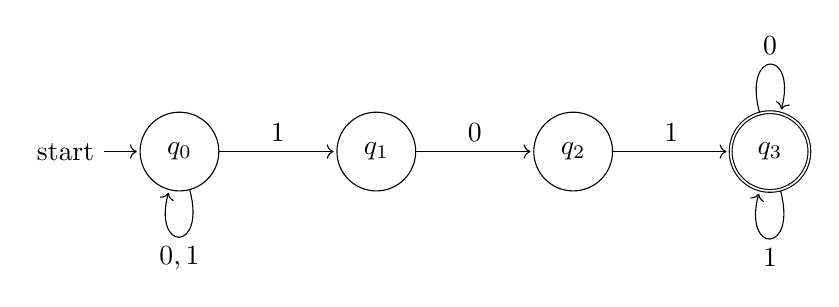
\begin{tikzpicture}[shorten >=1pt, node distance=2.5cm, auto,
    every state/.style={minimum size=1cm}]
  \node[state, initial] (q0) {$q_0$};
  \node[state] (q1) [right of=q0] {$q_1$};
  \node[state] (q2) [right of=q1] {$q_2$};
  \node[state, accepting] (q3) [right of=q2] {$q_3$};

  \path[->]
    (q0) edge [loop below] node {$0,1$} (q0)
    (q0) edge node {$1$} (q1)
    (q1) edge node {$0$} (q2)
    (q2) edge node {$1$} (q3)
    (q3) edge [loop above] node {$0$} (q3)
    (q3) edge [loop below] node {$1$} (q3);
\end{tikzpicture}
\]
Analizziamo ora il comportamento dell'automa su alcune parole:

\begin{itemize}
    \item Consideriamo la parola
    \[
    w=1101.
    \]
    Calcoliamo l'insieme degli stati raggiungibili dopo la lettura di ciascun simbolo:
    \[
    \begin{aligned}
    \widehat{T}(q_0,1)&=\{q_0,q_1\},\\
    \widehat{T}(q_0,11)
        &=T(q_0,1)\cup T(q_1,1)
        =\{q_0,q_1\}\cup\emptyset
        =\{q_0,q_1\},\\
    \widehat{T}(q_0,110)
        &=T(q_0,0)\cup T(q_1,0)
        =\{q_0\}\cup\{q_2\}
        =\{q_0,q_2\},\\
    \widehat{T}(q_0,1101)
        &=T(q_0,1)\cup T(q_2,1)
        =\{q_0,q_1\}\cup\{q_3\}
        =\{q_0,q_1,q_3\}.
    \end{aligned}
    \]
    Poiché l'insieme finale contiene lo stato finale $q_3$, la parola
    \[
    1101
    \]
    è accettata.

    \item Consideriamo ora la parola
    \[
    w=1000.
    \]
    Si ha
    \[
    \begin{aligned}
    \widehat{T}(q_0,1)&=\{q_0,q_1\},\\
    \widehat{T}(q_0,10)
        &=T(q_0,0)\cup T(q_1,0)
        =\{q_0\}\cup\{q_2\}
        =\{q_0,q_2\},\\
    \widehat{T}(q_0,100)
        &=T(q_0,0)\cup T(q_2,0)
        =\{q_0\}\cup\emptyset
        =\{q_0\},\\
    \widehat{T}(q_0,1000)
        &=T(q_0,0)
        =\{q_0\}.
    \end{aligned}
    \]
    L'insieme degli stati raggiungibili non contiene alcuno stato finale, quindi la parola
    \[
    1000
    \]
    è rifiutata.
    \item Consideriamo infine la parola
\[
w=1100101.
\]
Si ha
\[
\begin{aligned}
\widehat{T}(q_0,1)&=\{q_0,q_1\},\\
\widehat{T}(q_0,11)
    &=T(q_0,1)\cup T(q_1,1)
    =\{q_0,q_1\}\cup\emptyset
    =\{q_0,q_1\},\\
\widehat{T}(q_0,110)
    &=T(q_0,0)\cup T(q_1,0)
    =\{q_0\}\cup\{q_2\}
    =\{q_0,q_2\},\\
\widehat{T}(q_0,1100)
    &=T(q_0,0)\cup T(q_2,0)
    =\{q_0\}\cup\emptyset
    =\{q_0\},\\
\widehat{T}(q_0,11001)
    &=T(q_0,1)
    =\{q_0,q_1\},\\
\widehat{T}(q_0,110010)
    &=T(q_0,0)\cup T(q_1,0)
    =\{q_0\}\cup\{q_2\}
    =\{q_0,q_2\},\\
\widehat{T}(q_0,1100101)
    &=T(q_0,1)\cup T(q_2,1)
    =\{q_0,q_1\}\cup\{q_3\}
    =\{q_0,q_1,q_3\}.
\end{aligned}
\]
Poiché l'insieme finale contiene lo stato finale $q_3$, la parola
\[
1100101
\]
è accettata.
\end{itemize}
Si può mostrare infatti che questo automa è quello che decide l'insieme delle parole che contengono come sottostringa $101$.
Consideriamo ora lo stesso automa sostituendo la transizione
\[
T(q_0,1)=\{q_0,q_1\}
\]
con
\[
T(q_0,1)=\{q_1\},
\]
lasciando invariate tutte le altre transizioni.
Mostriamo che questo automa non riconosce più tutte le parole contenenti la sottostringa \(101\).
Infatti, la parola
\[
w=1101
\]
contiene la sottostringa \(101\), ma l'automa si comporta nel modo seguente:
\[
\begin{aligned}
\widehat{T}(q_0,\varepsilon)&=\{q_0\},\\
\widehat{T}(q_0,1)&=\{q_1\},\\
\widehat{T}(q_0,11)&=T(q_1,1)=\emptyset,\\
\widehat{T}(q_0,110)&=\bigcup_{q\in\emptyset}T(q,0)=\emptyset,\\
\widehat{T}(q_0,1101)&=\bigcup_{q\in\emptyset}T(q,1)=\emptyset.
\end{aligned}
\]
Poiché la computazione termina con l'insieme vuoto, la parola \(1101\) viene rifiutata.

L'errore consiste nel fatto che l'automa è costretto a scegliere il \emph{primo} simbolo \(1\) come possibile inizio della sottostringa \(101\). Nell'automa non deterministico originale, invece, il ramo che rimane nello stato \(q_0\) permette di ignorare il primo \(1\) e di scegliere il secondo \(1\) come inizio della sottostringa, accettando così correttamente la parola.
\end{exam}
In vista, dell'obiettivo di mostrare che l'insieme $X_1 \cdot X_2$ ottenuto a partire da due insiemi $X_1$ e $X_2$ DFA-decidibili è lui stesso DFA-decidibile dobbiamo poter costruire un automa che ``concatena'' la computazione di un automa con quella del secondo, a questo fine è comodo utilizzare una ulteriore variante della definizione di NDFA che può effettuare transizioni senza fare avanzare il puntatore alla posizione corrente:

\begin{defi}[Automa Finito non-deterministico con $\epsilon$-mosse]
\label{def:15}
Siano $A$ e $Q$ insiemi finiti, un automa finito non-deterministico con $\epsilon$-mosse \emph{di alfabeto $A$ e insieme degli stati $Q$} è una tripla $(T, q_0, F)$ dove
\[
T : Q \times A \cup \{\epsilon\} \to 2^Q
\]
\[
F \subset Q
\]
e $q_0 \in Q$ è uno stato particolare, detto \emph{stato iniziale}.
\end{defi}



Per la descrizione della computazione dovremo introdurre una variante della funzione di transizione che prenda in considerazione le $\epsilon$-mosse, a questo scopo introduciamo la seguente notazione per $S \in 2^Q$:
\[
T^k(S,a) :=
\begin{cases}
S & \text{se } k = 0 \\
T(T^{k-1}(S,a), a) & k > 0
\end{cases}
\]

\begin{defi}[Algoritmo associato ad un automa finito non-deterministico con $\epsilon$-mosse]
\label{def:17}
L'algoritmo associato ad un automa non-deterministico di alfabeto $A$ e insieme degli stati $Q$ viene descritto definendo le tre funzioni:
\begin{itemize}
\item la \textbf{funzione di ingresso} che associa ad un parola $w \in A^*$, la configurazione
\[
\varepsilon(w) = \left(w, 1, \bigcup_{k \geq 0} T^k(\{q_0\}, \epsilon)\right),
\]

\item la \textbf{funzione di transizione} $\tau : \mathrm{Conf}_{ND}^{A,Q} \to \mathrm{Conf}_{ND}^{A,Q}$ è data da
\[
\tau((w,p,S)) = \left(w, p+1, \bigcup_{k \geq 0} T^k(T(S, w(p)), \epsilon)\right),
\]

\item la \textbf{funzione di uscita} $\delta : \mathrm{Conf}_{ND}^{A,Q} \to \{0,1\}$, data da
\[
\delta((w,p,S)) =
\begin{cases}
0 & \text{se } p > |w| \text{ e } F \cap S = \emptyset \\
1 & \text{se } p > |w| \text{ e } F \cap S \neq \emptyset
\end{cases}
\]
\end{itemize}
\end{defi}


\begin{exam}[Un esempio di $\epsilon$-NDFA]
\label{es:16}

Consideriamo l'alfabeto
\[
A=\{0,1\},
\]
l'insieme degli stati
\[
Q=\{q_0,q_1,q_2,q_3\},
\]
e definiamo il seguente $\epsilon$-NDFA
\[
(T,q_0,F),
\]
dove
\[
F=\{q_3\}
\]
e
\[
T:Q\times(A\cup\{\epsilon\})\to 2^Q
\]
è definita da
\[
\begin{matrix}
T(q_0,0)&=&\{q_0\},\\
T(q_0,1)&=&\{q_0,q_1\},\\
T(q_1,0)&=&\{q_2\},\\
T(q_1,1)&=&\emptyset,\\
T(q_1,\epsilon)&=&\{q_2\},\\
T(q_2,0)&=&\emptyset,\\
T(q_2,1)&=&\{q_3\},\\
T(q_3,0)&=&\{q_3\},\\
T(q_3,1)&=&\{q_3\}.
\end{matrix}
\]
L'automa può essere rappresentato graficamente come
\[
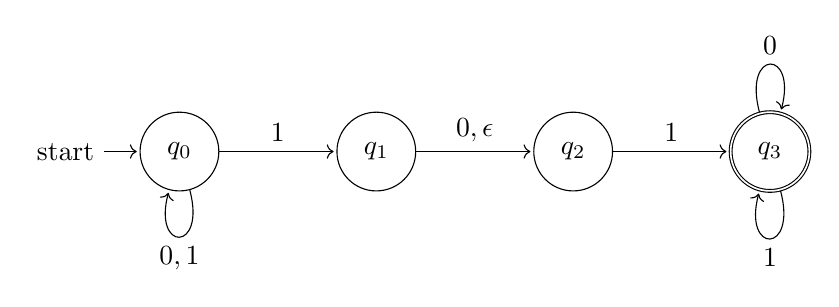
\begin{tikzpicture}[shorten >=1pt, node distance=2.5cm, auto,
    every state/.style={minimum size=1cm}]
  \node[state, initial] (q0) {$q_0$};
  \node[state] (q1) [right of=q0] {$q_1$};
  \node[state] (q2) [right of=q1] {$q_2$};
  \node[state, accepting] (q3) [right of=q2] {$q_3$};

  \path[->]
    (q0) edge [loop below] node {$0,1$} (q0)
    (q0) edge node {$1$} (q1)
    (q1) edge node {$0,\epsilon$} (q2)
    (q2) edge node {$1$} (q3)
    (q3) edge [loop above] node {$0$} (q3)
    (q3) edge [loop below] node {$1$} (q3);
\end{tikzpicture}
\]
Per descrivere la computazione consideriamo la funzione di transizione estesa
\[
\widehat{T}:2^Q\times A^*\to 2^Q
\]
definita considerando le $\epsilon$-mosse come transizioni gratuite. In
particolare, per ogni insieme di stati $S\subseteq Q$ poniamo
\[
T^0(S,\epsilon)=S,
\]
e
\[
T^k(S,\epsilon)=T(T^{k-1}(S,\epsilon),\epsilon)
\]
per $k>0$.
La computazione dell'automa consiste quindi nel considerare tutti gli stati
ottenibili dopo un numero finito di $\epsilon$-mosse.

\begin{itemize}

\item Consideriamo la parola
\[
w=101.
\]

Partendo dallo stato iniziale otteniamo
\[
\widehat{T}(q_0,\epsilon)=\{q_0\}.
\]

Dopo aver letto il primo simbolo $1$:
\[
T(\{q_0\},1)=\{q_0,q_1\}.
\]

Applicando successivamente le $\epsilon$-mosse:
\[
T^0(\{q_0,q_1\},\epsilon)=\{q_0,q_1\},
\]
\[
T^1(\{q_0,q_1\},\epsilon)
=
T(\{q_0,q_1\},\epsilon)
=
\{q_2\}.
\]

Quindi dopo il primo simbolo:
\[
\widehat{T}(q_0,1)
=
\{q_0,q_1,q_2\}.
\]

Ora leggiamo il simbolo $0$:
\[
T(\{q_0,q_1,q_2\},0)
=
\{q_0\}\cup\{q_2\}\cup\emptyset
=
\{q_0,q_2\}.
\]

Non sono possibili ulteriori $\epsilon$-mosse, quindi:
\[
\widehat{T}(q_0,10)=\{q_0,q_2\}.
\]

Infine leggiamo $1$:
\[
T(\{q_0,q_2\},1)
=
\{q_0,q_1\}\cup\{q_3\}
=
\{q_0,q_1,q_3\}.
\]

Poiché
\[
q_3\in\widehat{T}(q_0,101),
\]
la parola $101$ è accettata.

\item Consideriamo la parola
\[
w=10.
\]

Dopo il simbolo $1$ abbiamo già visto che
\[
\widehat{T}(q_0,1)=\{q_0,q_1,q_2\}.
\]

Leggendo $0$ otteniamo:
\[
T(\{q_0,q_1,q_2\},0)
=
\{q_0\}\cup\{q_2\}\cup\emptyset
=
\{q_0,q_2\}.
\]

Non essendo presente lo stato finale:
\[
q_3\notin\widehat{T}(q_0,10),
\]
la parola $10$ è rifiutata.

\end{itemize}

\end{exam}

Con la nozione appena introdotta è quindi possibile dimostrare in modo diretto che dati due insiemi NDFA-decidibili, l'insieme ottenuto come concatenazione è pure NDFA-decidibile, ovvero la Proposizione~\ref{prop:9} nel caso non-deterministico, e infatti
\begin{prop}
    Siano $X_1$ e $X_2$ decidibili per automa finito non-deterministico allora anche $X_1\cdot X_2$ è
decidibile per automa finito non-deterministico.
\begin{proof}
Siano i due automi che decidono $X_1 \subset A^*$ e $X_2 \subset A^*$ rispettivamente dati su insiemi degli stati disgiunti $Q_1$ e $Q_2$, ovvero con $Q_1 \cap Q_2 = \emptyset$: $\mathcal{A}_1 = (T', q_0', F')$ e $\mathcal{A}_2 = (T'', q_0'', F'')$.

Costruiamo l'automa che decide $X_1 \cdot X_2$ aggiungendo alle transizioni di $\mathcal{A}_1$ e $\mathcal{A}_2$ quelle che vanno dagli stati accettanti di $\mathcal{A}_1$ allo stato iniziale $q_0''$ del secondo automa, ovvero definiamo l'automa $\mathcal{A}$ con insieme degli stati $Q := Q_1 \cup Q_2$ dove lo stato iniziale è $q_0 := q_0' \in Q_1$ e gli stati finali accettanti sono definiti come quelli di $\mathcal{A}_2$, dunque:
\[
\mathcal{A} := (T, q_0, F)
\]
dove
\[
T(q,a) :=
\begin{cases}
T'(q,a) & \text{se } q \in F' \text{ e } a \neq \epsilon \text{ oppure } q \notin F', \\
T'(q,a) \cup \{q_0''\} & q \in F' \text{ e } a = \epsilon, \\
T''(q,a) & q \in Q_2,
\end{cases}
\]
e l'insieme degli stati finali accettanti è dato da $F := F''$.
\end{proof} 
\end{prop}
\begin{prop}
\label{prop:19}
Sia dato un insieme $X \subseteq A^*$ per un certo alfabeto finito $A$.
Allora
\[
X \text{ è DFA-decidibile}
\iff
X \text{ è NDFA-decidibile}
\iff
X \text{ è }\epsilon\text{-NDFA-decidibile}.
\]

\begin{proof}
Procediamo dimostrando le tre implicazioni.

\begin{itemize}

\item[$(\mathrm{DFA}\Rightarrow\mathrm{NDFA})$]
Sia $(T,q_0,F)$ un DFA. Basta considerare la funzione di transizione come funzione a valori nell'insieme delle parti:
\[
T' : Q\times A\longrightarrow 2^Q,
\]
definita da
\[
T'(q,a):=\{T(q,a)\}.
\]
L'automa così ottenuto è un NDFA che produce esattamente la stessa computazione.

\item[$(\mathrm{NDFA}\Rightarrow\epsilon\text{-}\mathrm{NDFA})$]
Sia $(T,q_0,F)$ un NDFA. Definiamo
\[
T':Q\times(A\cup\{\epsilon\})\longrightarrow 2^Q
\]
ponendo
\[
T'(q,a):=T(q,a),
\qquad
a\in A,
\]
e
\[
T'(q,\epsilon):=\varnothing.
\]
In questo modo l'automa non utilizza mai $\epsilon$-mosse e coincide con quello di partenza.

\item[$(\epsilon\text{-}\mathrm{NDFA}\Rightarrow\mathrm{DFA})$]
Sia $(T,q_0,F)$ un $\epsilon$-NDFA.

Consideriamo come insieme degli stati
\[
Q'=2^Q.
\]

La funzione di transizione del DFA è definita da
\[
T':2^Q\times A\longrightarrow 2^Q,
\]
ponendo
\[
T'(S,a):=
\bigcup_{k\ge0}
T^k(T(S,a),\epsilon).
\]

Lo stato iniziale è
\[
q_0':=
\bigcup_{k\ge0}
T^k(\{q_0\},\epsilon),
\]
mentre l'insieme degli stati finali è
\[
F':=
\{\,S\subseteq Q\mid S\cap F\neq\varnothing\,\}.
\]

È facile controllare che per ogni parola $\omega$ le computazioni ottenute tramite i rispettivi algoritmi coincidono, pertanto le decisioni dei due automi coincideranno per ogni $\omega$ e quindi decideranno lo stesso
insieme.

\end{itemize}

Ne segue che le tre nozioni di decidibilità coincidono.
\end{proof}
\end{prop}
\newpage
\section{Espressioni regolari}
Avendo individuato i costrutti rispetto ai quali l’insieme di tutti gli insiemi regolari resta invariato (concatenazione, unione e operatore * di Kleene), si può formalizzare una grammatica data dalla rappresentazione
simbolica di alcuni insiemi regolari di base.
\begin{defi}
    Fissiamo un alfabeto $A$. L'insieme $\mathcal E$ (anche indicato con $E$) delle \textit{espressioni regolari} sull'alfabeto 
$A$ è il più piccolo insieme tale che: 
\begin{itemize}
    \item $\mathbb  0, \mathbb 1 \in \mathcal E$;

    \item  per ogni $a \in A$ $a \in \mathcal E$;

    \item se $E_1, E_2 \in \mathcal E $ allora 
    \(
    E_1 + E_2,
    E_1 \cdot E_2,
    E_1^*\in \mathcal E
    \)
\end{itemize}
\end{defi}
\begin{exam}
    Alcune espressioni regolari sull’alfabeto $A= {0,1}$ sono:
    \begin{itemize}
        \item $\mathbb 0$;

        \item $\mathbb 0+0$;

        \item $(0+1)^*$;

        \item $0\cdot (0+1\cdot 1)^*\cdot \mathbb 1$.
    \end{itemize}
\end{exam}
\begin{rema}
    Chiaramente, fino ad ora, abbiamo usato i simboli $+,\cdot, \cdot$ in due contesti diversi: per la definizione formale di espressione regolare e per le definizioni di operazioni sui sottoinsiemi degli alfabeti.
    Questo non è un problema visto che si capisce a quale definizione si fa riferimento in base al contesto.
\end{rema}
\begin{defi}[Interpretazione di un'espressione regolare]
\label{def:22}
Per ogni espressione regolare $e\in E$, di alfabeto $A$, definiamo un'interpretazione
\[
\llbracket\ \rrbracket : E \longrightarrow 2^{A^*}
\]
dove
\[
\llbracket e\rrbracket :=
\left\{
\begin{matrix}
\varnothing & \text{se } e=\mathbb{0} & \text{(insieme vuoto)}\\[2pt]
\{\epsilon\} & \text{se } e=\mathbb{1} & \text{(insieme singleton parola vuota)}\\[2pt]
\{a\} & \text{se } e=a\in A & \text{(insieme singleton simbolo)}\\[2pt]
\llbracket e_1\rrbracket\cdot\llbracket e_2\rrbracket & \text{se } e=e_1\cdot e_2 & \text{(concatenazione)}\\[2pt]
\llbracket e_1\rrbracket+\llbracket e_2\rrbracket & \text{se } e=e_1+e_2 & \text{(unione)}\\[2pt]
\llbracket e_1\rrbracket^* & \text{se } e=e_1^* & \text{(insieme star)}
\end{matrix}
\right.
\]
\end{defi}
\begin{figure}[H]
\centering
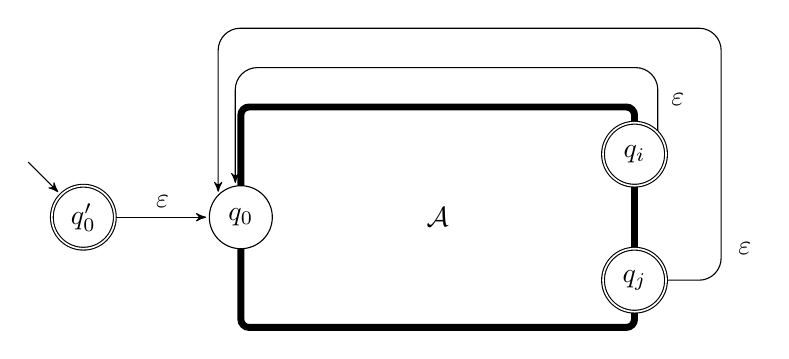
\begin{tikzpicture}[
    >=stealth', shorten >=1pt, auto,
    every state/.style={circle, draw, fill=white, minimum size=0.8cm, inner sep=1pt}
]
% Rettangolo di A
\draw[-, line width=2.5pt, rounded corners=3pt] (2,-1.4) rectangle (7,1.4);
\node at (4.5,0) {$\mathcal{A}$};

% Stati (q_0 ora sul bordo sinistro, in sovrimpressione)
\node[state, accepting] (q0p) at (0,0)    {$q_0'$};
\node[state]            (q0)  at (2,0)    {$q_0$};
\node[state, accepting] (qi)  at (7,0.8)  {$q_i$};
\node[state, accepting] (qj)  at (7,-0.8) {$q_j$};

% Freccia d'ingresso e epsilon-mossa iniziale
\draw[->] ([shift={(-0.7,0.7)}]q0p.center) -- (q0p);
\draw[->] (q0p) -- node {$\varepsilon$} (q0);

% epsilon-mossa di ritorno interna (da q_i)
\draw[->, rounded corners=8pt]
    (qi.45) -- (qi.45 |- 0,1.9) -- (q0.100 |- 0,1.9) -- (q0.100);
\node at (7.55,1.5) {$\varepsilon$};

% epsilon-mossa di ritorno esterna (da q_j)
\draw[->, rounded corners=8pt]
    (qj.0) -- (8.1,-0.8) -- (8.1,2.4) -- (q0.135 |- 0,2.4) -- (q0.135);
\node at (8.4,-0.4) {$\varepsilon$};
\end{tikzpicture}
\caption{Costruzione dell'automa che decide $X^*$ a partire da quello che decide $X$.}
\label{fig:kleene}
\end{figure}

\begin{rema}
    Chiaramente, riprendendo la precedente osservazione, con $\llbracket e_1\rrbracket\cdot\llbracket e_2\rrbracket$ indichiamo la conatenazione degli insiemi $\llbracket e_1\rrbracket$ e $\llbracket e_2\rrbracket$.
\end{rema}

\begin{prop} Data un’espressione regolare $e\in E$ l’insieme $\llbracket e \rrbracket$ è un insieme regolare.
\begin{proof} Questo risultato è conseguenza delle proprietà di chiusura (per prodotto, somma e star)
soddisfatte dagli insiemi DFA-decidibili, e dal fatto che le tre espressioni regolari di base si interpretano
con insiemi DFA-decidibili: si veda la figura 
\ref{fig:automi-base} per gli automi che decidono le tre espressioni regolari di base.
\end{proof}
\end{prop}
\begin{figure}[H]
\centering
\begin{subfigure}[t]{0.3\textwidth}
    \centering
    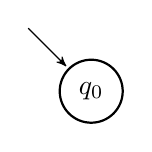
\begin{tikzpicture}[
        ->, >=stealth', shorten >=1pt, auto, node distance=3cm,
        every state/.style={circle, draw, thick, minimum size=0.8cm, inner sep=1pt}
    ]
    \node[state] (q0) {$q_0$};
    \draw[->] ([shift={(-0.8,0.8)}]q0.center) -- (q0);
    \end{tikzpicture}
    \caption{NDFA che decide l'insieme vuoto}
    \label{fig:ndfa-vuoto}
\end{subfigure}
\hfill
\begin{subfigure}[t]{0.3\textwidth}
    \centering
    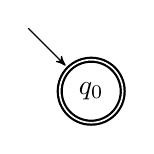
\begin{tikzpicture}[
        ->, >=stealth', shorten >=1pt, auto, node distance=3cm,
        every state/.style={circle, draw, thick, minimum size=0.8cm, inner sep=1pt}
    ]
    \node[state, accepting] (q0) {$q_0$};
    \draw[->] ([shift={(-0.8,0.8)}]q0.center) -- (q0);
    \end{tikzpicture}
    \caption{NDFA che decide l'insieme singleton della parola vuota}
    \label{fig:ndfa-epsilon}
\end{subfigure}
\hfill
\begin{subfigure}[t]{0.36\textwidth}
    \centering
    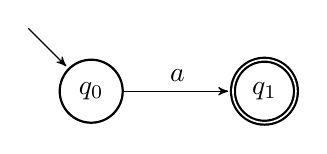
\begin{tikzpicture}[
        ->, >=stealth', shorten >=1pt, auto, node distance=2.2cm,
        every state/.style={circle, draw, thick, minimum size=0.8cm, inner sep=1pt}
    ]
    \node[state] (q0) {$q_0$};
    \node[state, accepting] (q1) [right of=q0] {$q_1$};
    \draw[->] ([shift={(-0.8,0.8)}]q0.center) -- (q0);
    \path (q0) edge node {$a$} (q1);
    \end{tikzpicture}
    \caption{NDFA che decide l'insieme singleton di una lettera dell'alfabeto}
    \label{fig:ndfa-lettera}
\end{subfigure}
\caption{Gli automi che decidono le tre espressioni regolari di base}
\label{fig:automi-base}
\end{figure}
\begin{figure}[H]
\centering
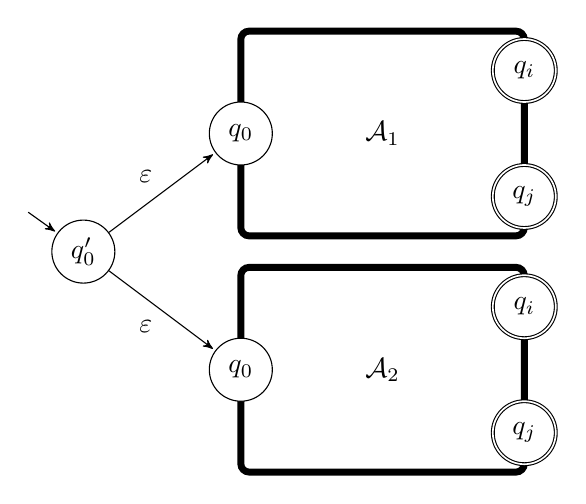
\begin{tikzpicture}[
    >=stealth', shorten >=1pt, auto,
    every state/.style={circle, draw, fill=white, minimum size=0.8cm, inner sep=1pt}
]
% Automa A1 (sopra)
\draw[-, line width=2.5pt, rounded corners=3pt] (3,0.2) rectangle (6.6,2.8);
\node at (4.8,1.5) {$\mathcal{A}_1$};
\node[state] (q0a) at (3,1.5) {$q_0$};
\node[state, accepting] (qia) at (6.6,2.3) {$q_i$};
\node[state, accepting] (qja) at (6.6,0.7) {$q_j$};

% Automa A2 (sotto)
\draw[-, line width=2.5pt, rounded corners=3pt] (3,-2.8) rectangle (6.6,-0.2);
\node at (4.8,-1.5) {$\mathcal{A}_2$};
\node[state] (q0b) at (3,-1.5) {$q_0$};
\node[state, accepting] (qib) at (6.6,-0.7) {$q_i$};
\node[state, accepting] (qjb) at (6.6,-2.3) {$q_j$};

% Nuovo stato iniziale
\node[state] (q0p) at (1,0) {$q_0'$};
\draw[->] ([shift={(-0.7,0.5)}]q0p.center) -- (q0p);

% epsilon-mosse
\draw[->] (q0p) -- node[above left, pos=0.5] {$\varepsilon$} (q0a);
\draw[->] (q0p) -- node[below left, pos=0.5] {$\varepsilon$} (q0b);
\end{tikzpicture}
\caption{Costruzione dell'automa che decide $X_1 + X_2$ a partire da quelli che decidono $X_1$ e $X_2$.}
\label{fig:somma}
\end{figure}
Quello che invece vorremmo mostrare ora è che vale anche l'implicazione inversa della proposizione precedente. Per farlo introdurremo una nuova versione di automa.
\begin{defi}
Un \textit{automa a stati finiti non-deterministico generalizzato} di alfabeto $A$ e insieme degli stati $Q$ è una tripla:
\[
(T, q_0, F)
\]
dove
\[
T : Q \times E \to 2^Q,
\]
$q_0 \in Q$ è detto stato iniziale, $F \subset Q$ è detto insieme degli stati finali accettanti.
\end{defi}
L'idea alla base di questo nuovo tipo di automa è
che si può etichettare le transizioni dell'automa
non solo con le lettere dell'alfabeto ma con
qualsiasi espressione costruita a partire dall'alfabeto.
A questo punto, dovremmo però dare di nuovo le definizioni di
algoritmo associato ad un automa generalizzato e di decidibilità.
Usando però la proposizione sopra, possiamo fare ciò in modo furbo:
\begin{rema}
    \label{aut generalizzato a eps. NDFA}
    Dato un automa generalizzato $A=(T,q_0,F)$ con insieme di stati $Q$,
    gli si può associare un $\epsilon$-NDFA nel seguente modo.
    Per ogni coppia $(q,e)$ tale che
    $T(q,e)=p$,
    il risultato precedente fornisce un DFA $A_e=(T^e, q_0^e, F^e)$
    che decide l'iniseme regolare $\llbracket e \rrbracket$.
    A questo punto, possiamo modificare l'automa $A$ in un $\epsilon$-NDFA della forma $A'=(T', q_0', F')$, 
    eliminando tutte le definizioni del tipo
    $T(q,e)=p$ e aggiungendo per ogni coppia $(q,e)$ come sopra:
    \begin{enumerate}
        \item una $\epsilon$-transizione
        che collega $q$ a $q_0^e$, ovvero definendo $T'(q,\epsilon):=q_0$;

        \item le transizioni interne di ogni $A_e$;
        
        \item una $\epsilon$-transizione
        che collega ogni stato accettante di $A_e$ $q_i$ a $p$, ovvero definendo $T'(q_i,\epsilon):=p$ per ogni $q_i\in F^e$.
    \end{enumerate}
\end{rema}
\begin{figure}[H]
\centering
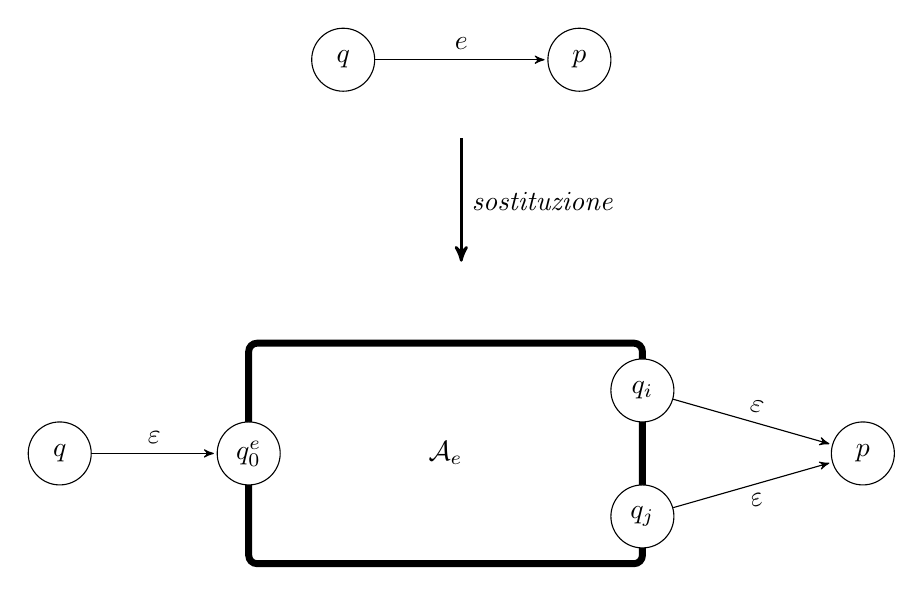
\begin{tikzpicture}[
    >=stealth', shorten >=1pt, auto,
    every state/.style={circle, draw, fill=white, minimum size=0.8cm, inner sep=1pt}
]
%%%%%%%%%%%%%%%%%%%% Automa di partenza %%%%%%%%%%%%%%%%%%%%
% Stati
\node[state] (q) at (3.6,0) {$q$};
\node[state] (p) at (6.6,0) {$p$};

% Transizione T(q,e) = p
\draw[->] (q) -- node {$e$} (p);

%%%%%%%%%%%%%%%%%%%% Freccia di trasformazione %%%%%%%%%%%%%%%%%%%%
\draw[->, line width=1pt] (5.1,-1) -- node[right] {\textit{sostituzione}} (5.1,-2.6);

%%%%%%%%%%%%%%%%%%%% Automa trasformato %%%%%%%%%%%%%%%%%%%%
% Rettangolo di A_e
\draw[-, line width=2.5pt, rounded corners=3pt] (2.4,-6.4) rectangle (7.4,-3.6);
\node at (4.9,-5) {$\mathcal{A}_e$};

% Stati
\node[state] (qb)  at (0,-5)     {$q$};
\node[state] (q0e) at (2.4,-5)   {$q_0^e$};
\node[state] (qi)  at (7.4,-4.2) {$q_i$};
\node[state] (qj)  at (7.4,-5.8) {$q_j$};
\node[state] (pb)  at (10.2,-5)  {$p$};

% epsilon-mossa di ingresso in A_e
\draw[->] (qb) -- node {$\varepsilon$} (q0e);

% epsilon-mosse di uscita dagli stati accettanti di A_e
\draw[->] (qi) -- node[above, sloped] {$\varepsilon$} (pb);
\draw[->] (qj) -- node[below, sloped] {$\varepsilon$} (pb);
\end{tikzpicture}
\caption{Un passo di sostituzione: la transizione $T(q,e)=p$ viene rimpiazzata dal DFA $\mathcal{A}_e$ che decide $\llbracket e \rrbracket$, collegato a $q$ e a $p$ tramite $\varepsilon$-transizioni.}
\label{fig:sostituzione}
\end{figure}
\begin{defi}
    Dato un automa generalizzato $A$, \textit{l'insieme $X \subset A^*$
    deciso dall'automa generalizzato $A$} è l'insieme deciso dall'$\epsilon$-NDFA
    che gli si può associare usando la procedura esposta nell'osservazione \ref{aut generalizzato a eps. NDFA}.
\end{defi}
Ora elenchiamo tre trasformazioni 
che si possono effettuare su un automa generalizzato
che non modicano l'insieme deciso dall'automa stesso.
\begin{itemize}
    \item Setup restituisce l'automa con l'aggiunta di uno stato iniziale $q_0^*$ e di un unico stato finale $q_F^*$ che non hanno archi entranti e su cui non saranno fatte agire le trasformazioni seguenti (Merge e Erase). Il nuovo automa avrà le stesse transizioni dell'automa dato con l'aggiunta di una $\epsilon$-transizione da $q_0^*$ a $q_0$ e di $\epsilon$-transizioni da ogni \textcolor{red}{Queste epsilon mosse non dovrebbero essere delle $\mathbb 1$-mosse visto che stiamo eticchettando con le espressioni.} stato finale $q \in F$ verso $q_F^*$:
    \[
    T'(q, e) := 
    \begin{cases} 
    q_0 & \text{se } q = q_0^* \text{ e } e = \epsilon \\ 
    q_F^* & \text{se } q \in F \text{ e } e = \epsilon \\ 
    T(q, e) & \text{altrimenti.} 
    \end{cases}
    \]

    \begin{figure}[H]
\centering
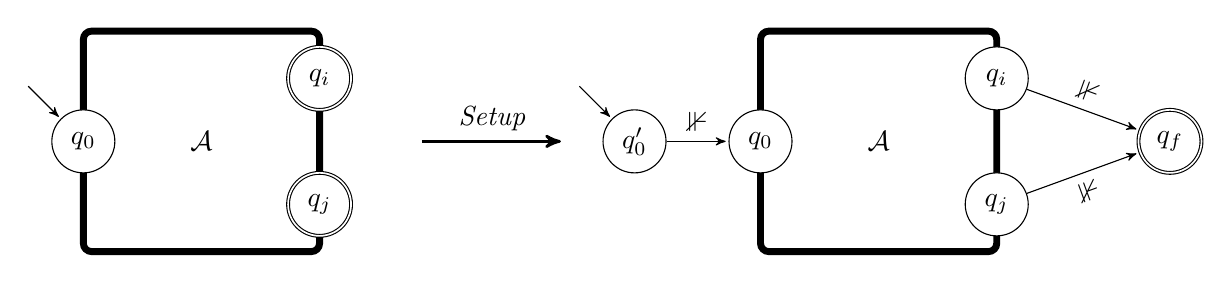
\begin{tikzpicture}[
    >=stealth', shorten >=1pt, auto,
    every state/.style={circle, draw, fill=white, minimum size=0.8cm, inner sep=1pt}
]
%%%%%%%%%%%%%%%%%%%% Automa di partenza %%%%%%%%%%%%%%%%%%%%
% Rettangolo di A
\draw[-, line width=2.5pt, rounded corners=3pt] (0,-1.4) rectangle (3,1.4);
\node at (1.5,0) {$\mathcal{A}$};

% Stati
\node[state]            (q0)  at (0,0)    {$q_0$};
\node[state, accepting] (qi)  at (3,0.8)  {$q_i$};
\node[state, accepting] (qj)  at (3,-0.8) {$q_j$};

% Freccia d'ingresso
\draw[->] ([shift={(-0.7,0.7)}]q0.center) -- (q0);

%%%%%%%%%%%%%%%%%%%% Freccia di trasformazione %%%%%%%%%%%%%%%%%%%%
\draw[->, line width=1pt] (4.3,0) -- node[above] {\textit{Setup}} (6.1,0);

%%%%%%%%%%%%%%%%%%%% Automa trasformato %%%%%%%%%%%%%%%%%%%%
% Rettangolo di A
\draw[-, line width=2.5pt, rounded corners=3pt] (8.6,-1.4) rectangle (11.6,1.4);
\node at (10.1,0) {$\mathcal{A}$};

% Stati
\node[state]            (q0p) at (7,0)      {$q_0'$};
\node[state]            (q0b) at (8.6,0)    {$q_0$};
\node[state]            (qib) at (11.6,0.8) {$q_i$};
\node[state]            (qjb) at (11.6,-0.8){$q_j$};
\node[state, accepting] (qf)  at (13.8,0)   {$q_f$};

% Freccia d'ingresso e epsilon-mossa iniziale
\draw[->] ([shift={(-0.7,0.7)}]q0p.center) -- (q0p);
\draw[->] (q0p) -- node {$\mathbb 1$} (q0b);

% epsilon-mosse verso il nuovo stato finale
\draw[->] (qib) -- node[above, sloped] {$\mathbb 1$} (qf);
\draw[->] (qjb) -- node[below, sloped] {$\mathbb 1$} (qf);
\end{tikzpicture}
\caption{Trasformazione dell'automa $\mathcal{A}$ dopo Setup.}
\label{fig:setup}
\end{figure}

    \item Merge restituisce l'automa in cui due transizioni parallele sono fuse in un'unica transizione: in pratica, poiché l'automa generalizzato è non deterministico è possibile avere due espressioni $e_1$ ed $e_2$ tali che $T(q_i, e_1) = s_1$ e $T(q_i, e_2) = s_2$ e $q_j \in s_1 \cap s_2$. Sono queste due transizioni, dette \textit{parallele} per la coppia di stati $(q_i, q_j)$, che possono essere fuse in un'unica transizione in corrispondenza della somma delle due espressioni regolari.
    
    Definiamo l'automa $(T', q_0, F)$ in cui le transizioni da $q_i$ a $q_j$ sono sostituite con un'unica transizione $T' := \text{Merge}(T, q_i, q_j)$:
    \[
    T'(q, e) = 
    \begin{cases} 
    T(q, e) & \text{se } q \neq q_i \text{ e } T(q, e) \neq q_j \\ 
    \displaystyle \sum_{e \in E_{i,j}} e & \text{se } E_{i,j} := \{e \mid q = q_i \text{ e } T(q_i, e) = q_j\} 
    \end{cases}
    \]

\begin{figure}[H]
\centering
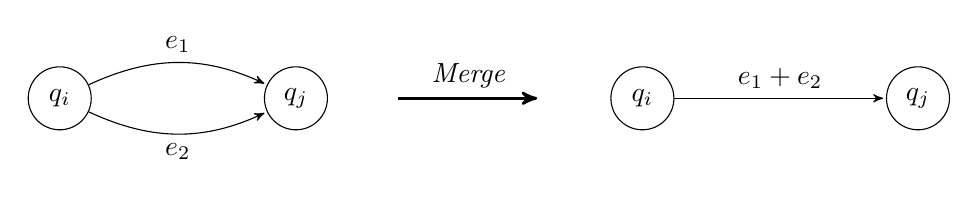
\begin{tikzpicture}[
    >=stealth', shorten >=1pt, auto,
    every state/.style={circle, draw, fill=white, minimum size=0.8cm, inner sep=1pt}
]
%%%%%%%%%%%%%%%%%%%% Automa di partenza %%%%%%%%%%%%%%%%%%%%
% Stati
\node[state] (qi)  at (0,0) {$q_i$};
\node[state] (qj)  at (3,0) {$q_j$};

% Transizioni parallele
\draw[->] (qi) to[bend left=25]  node {$e_1$} (qj);
\draw[->] (qi) to[bend right=25] node[below] {$e_2$} (qj);

%%%%%%%%%%%%%%%%%%%% Freccia di trasformazione %%%%%%%%%%%%%%%%%%%%
\draw[->, line width=1pt] (4.3,0) -- node[above] {\textit{Merge}} (6.1,0);

%%%%%%%%%%%%%%%%%%%% Automa trasformato %%%%%%%%%%%%%%%%%%%%
% Stati
\node[state] (qib) at (7.4,0)  {$q_i$};
\node[state] (qjb) at (10.9,0) {$q_j$};

% Transizione unica
\draw[->] (qib) -- node {$e_1 + e_2$} (qjb);
\end{tikzpicture}
\caption{Fusione di due transizioni parallele da $q_i$ a $q_j$ in un'unica transizione etichettata dalla somma delle espressioni regolari.}
\label{fig:merge}
\end{figure}
\begin{figure}[H]
\centering
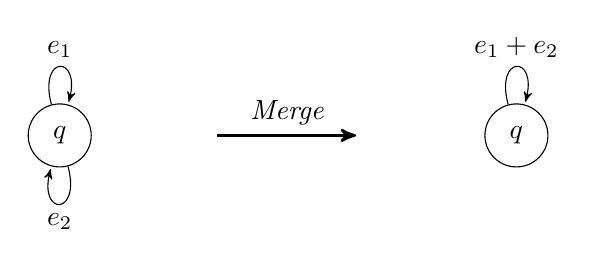
\begin{tikzpicture}[
    >=stealth', shorten >=1pt, auto,
    every state/.style={circle, draw, fill=white, minimum size=0.8cm, inner sep=1pt}
]
%%%%%%%%%%%%%%%%%%%% Automa di partenza %%%%%%%%%%%%%%%%%%%%
% Stato
\node[state] (q) at (0,0) {$q$};

% Loop paralleli (archi paralleli da q a q)
\draw[->] (q) edge[loop above] node {$e_1$} (q);
\draw[->] (q) edge[loop below] node {$e_2$} (q);

%%%%%%%%%%%%%%%%%%%% Freccia di trasformazione %%%%%%%%%%%%%%%%%%%%
\draw[->, line width=1pt] (2.0,0) -- node[above] {\textit{Merge}} (3.8,0);

%%%%%%%%%%%%%%%%%%%% Automa trasformato %%%%%%%%%%%%%%%%%%%%
% Stato
\node[state] (qb) at (5.8,0) {$q$};

% Loop unico
\draw[->] (qb) edge[loop above] node {$e_1 + e_2$} (qb);
\end{tikzpicture}
\caption{Caso particolare del Merge con $q_i = q_j = q$: due cappi su $q$ sono transizioni parallele da $q$ a $q$, e vengono fusi in un unico cappio etichettato da $e_1 + e_2$.}
\label{fig:merge-loop}
\end{figure}

    \item Erase Consideriamo un automa generalizzato $(T, q_0, F)$ senza transizioni parallele e introduciamo la seguente trasformazione che consiste nell'eliminare uno stato $\bar{q} \notin F \cup \{q_0\}$ preservando l'insieme che viene deciso dall'automa: il nuovo automa $(T', q_0, F)$ sarà dunque definito su $Q \setminus \{\bar{q}\}$ nel modo seguente: 
    
    se $T(q_i, e_i) = \bar{q}$, $T(\bar{q}, e_j) = q_j$ e $T(\bar{q}, e_k) = \bar{q}$ allora
    \[
    T'(q_i, e) = q_j \text{ dove } e = e_i e_k^* e_j
    \]
    
    per tutte le altre transizioni che non coinvolgono $\bar{q}$ non si interviene e si definisce
    \[
    T'(q, e) = T(q, e).
    \]
\begin{figure}[H]
\centering
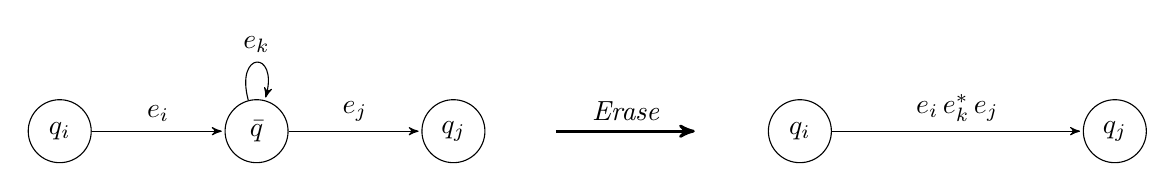
\begin{tikzpicture}[
    >=stealth', shorten >=1pt, auto,
    every state/.style={circle, draw, fill=white, minimum size=0.8cm, inner sep=1pt}
]
%%%%%%%%%%%%%%%%%%%% Automa di partenza %%%%%%%%%%%%%%%%%%%%
% Stati
\node[state] (qi) at (0,0) {$q_i$};
\node[state] (qb) at (2.5,0) {$\bar q$};
\node[state] (qj) at (5,0) {$q_j$};

% Transizioni
\draw[->] (qi) -- node {$e_i$} (qb);
\draw[->] (qb) -- node {$e_j$} (qj);
\draw[->] (qb) edge[loop above] node {$e_k$} (qb);

%%%%%%%%%%%%%%%%%%%% Freccia di trasformazione %%%%%%%%%%%%%%%%%%%%
\draw[->, line width=1pt] (6.3,0) -- node[above] {\textit{Erase}} (8.1,0);

%%%%%%%%%%%%%%%%%%%% Automa trasformato %%%%%%%%%%%%%%%%%%%%
% Stati
\node[state] (qib) at (9.4,0)  {$q_i$};
\node[state] (qjb) at (13.4,0) {$q_j$};

% Transizione unica
\draw[->] (qib) -- node {$e_i\, e_k^{*}\, e_j$} (qjb);
\end{tikzpicture}
\caption{Eliminazione dello stato $\bar q$: il cammino $q_i \to \bar q \to q_j$ con cappio su $\bar q$ diventa un'unica transizione etichettata da $e_i e_k^* e_j$.}
\label{fig:erase}
\end{figure}
\end{itemize}
A questo punto
possiamo mostrare il seguente risultato.
\begin{prop}
    Dato $X$ un isnieme regolare, 
    esiste un'espressione regolare 
    $e_X$ tale che
    $\llbracket e_X \rrbracket = X$.
    \begin{proof}
        Consideriamo $A$ un DFA che decide $X$.
        Consideriamo l'automa generalizzato $A'$ definito partendo da $A$
        e considerando come etichette gli elementi formali di 
        del linguaggio $E_A$ invece che le lettere di $A$.
        A questo punto abbiamo un automa generalizzato e possiamo applicare l'operazione "Setup"
        e poi le operazioni "Merge" e "Erase"
        fino a quando non otteniamo un automa con solo due stati, $q_0^*$ e $q_F^*$
        (quelli introdotti con l'operazione "Setup") e un solo arco tra i due stati etichettato 
        con l'espressione $e$.
        Usando che le operazioni sugli automi generalizzati definite prima non modificano l'insieme deciso,
        otteniamo che $e_X=e$.
    \end{proof}
\end{prop}

\newpage

\section{Macchina di Turing}
\subsection{Configurazione e algoritmo associato}
Alla luce di quanto fatto prima, sembrerebbe naturale chiamare algoritmica qualsiasi procedura costruita a partire da un
automa finito.
In particolare è chiaro che una tale procedura può essere descritta in un linguaggio di
programmazione e implementata in un qualsiasi sistema informatico. L’affermazione reciproca al contrario
sembrerebbe troppo restrittiva: non sembra difendibile che ogni procedura che si voglia definire algoritmica
debba essere realizzata mediante il modello di algoritmi associato agli automi finiti (più avanti vederemo degli esempi). 
Abolire completamente il carattere finito dell’insieme degli stati
svuoterebbe di significato la nozione stessa di algoritmo. Un algoritmo è, per definizione, una procedura descritta da un insieme finito di istruzioni/regole — è proprio questo che lo rende "eseguibile", trascrivibile, comunicabile, implementabile in un programma. Se l'insieme degli stati fosse infinito, la "macchina" non sarebbe più descrivibile con una quantità finita di dati.
Per conservare il carattere finitario auspicato senza rinunciare a fondamentali
capacità di calcolo, si può prescindere dal principio che l’automa non modifica la parola iniziale, dunque nel
leggere un certo simbolo dalla memoria potrà successivamente utilizzare questa informazione per modificare il
proprio stato ma anche per modificare la memoria scrivendo sulla stessa un nuovo carattere.
Questa variante
risulta interessante solo se a sua volta lo scorrimento automatico dei caratteri in lettura viene modificato per
permettere alla macchina di riesaminare i caratteri che sono stati modificati nei passi di calcolo precedenti,
altrimenti la modifica che permette di scrivere non avrebbe alcun impatto sul calcolo effettuato.
\begin{exam}
Consideriamo lgli insiemi
\[
X_0=
\{
0^n1^m \, | \, n,m \in \mathbb N
\},
\quad
X_1=
\{
0^n1^n \, | \, n \in \mathbb N
\} 
\]
Sebbene $X_0$ sia un insieme DFA-decidibile,
$X_1$ non lo è.
Infatti
gli automi non sono in grando di "contare",
quindi non si potrebbe contare il numero di occorenze di
$1$ e $0$
(forniremo una dimostrazione più avanti).
\end{exam}
\begin{figure}[H]
\centering
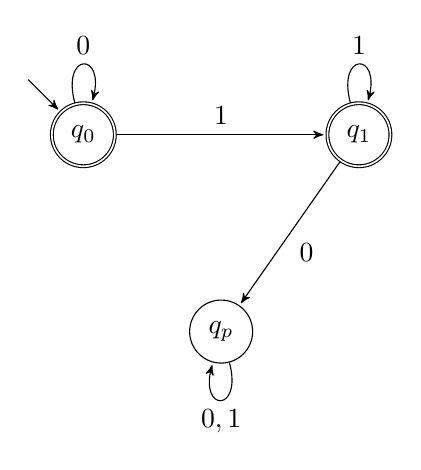
\begin{tikzpicture}[
    >=stealth', shorten >=1pt, auto,
    every state/.style={circle, draw, fill=white, minimum size=0.8cm, inner sep=1pt}
]
% Stati
\node[state, accepting] (q0) at (0,0)    {$q_0$};
\node[state, accepting] (q1) at (3.5,0)  {$q_1$};
\node[state]            (qp) at (1.75,-2.5) {$q_p$};

% Freccia d'ingresso
\draw[->] ([shift={(-0.7,0.7)}]q0.center) -- (q0);

% Transizioni
\draw[->] (q0) -- node {$1$} (q1);
\draw[->] (q1) -- node {$0$} (qp);

% Cappi
\path[->] (q0) edge[loop above] node {$0$}    (q0);
\path[->] (q1) edge[loop above] node {$1$}    (q1);
\path[->] (qp) edge[loop below] node {$0,1$}  (qp);
\end{tikzpicture}
\caption{DFA che decide il linguaggio $\{0^n1^m \mid n,m\in\mathbb N\}$.}
\label{fig:dfa-0n1m}
\end{figure}
In questa sezione vogliamo introdurre un modello
di calcolo più forte degli automi.
\begin{defi} Una \emph{configurazione ad un nastro di alfabeto $A$ e insieme degli stati $Q$} è una tripla $(f,p,q)$, dove
\begin{enumerate}
\item il \textit{nastro} è una funzione $f : \mathbb{Z} \to A'$ dove $A' := A \cup \{\square\}$ (a volte indicato anche con $\tilde{A}$) e tale che $|f^{-1}(A)| < \infty$,
\item $p \in \mathbb{Z}$,
\item $q \in Q'$ dove $Q' = Q \cup \{q_F^0, q_F^1\}$ essendo $q_F^0$ e $q_F^1$ due stati che non appartengono a $Q$.
\end{enumerate}

L'insieme delle configurazioni per un nastro di alfabeto $A$ e insieme degli stati $Q$ sarà denotato con
\[
Conf_1^{A,Q} := \{(f,p,q) \text{ che verificano i punti {(1)}, {(2)}, e {(3)}}\}
\]

\end{defi}
Il criterio di arresto, che questa volta non è determinato dalla fine della lettura del nastro, deve essere
specificato esplicitamente utilizzando un certo numero di stati terminali, che nella definizione sopra sono $q_F^0$ e $q_F^1$.
Bisogna inoltre fissare uno stato particolare da utilizzare per la codifica della configurazione iniziale a partire dalla parola di ingresso. Questo stato iniziale indicato da $q_0 \in  Q$ determina allora la configurazione
iniziale tramite una funzione di input $\epsilon()$.
Lo stato iniziale sarà d’ora in poi indicato da $q_0$.
\begin{defi}[Machcina di Turing]
     Dato un alfabeto $A$ e un insieme finito di stati $Q$, la \emph{macchina di Turing di alfabeto $A$ e stati $Q$} è un'applicazione
\[
\mu : Q \times \tilde{A} \to Q' \times \tilde{A} \times \{+1,-1\}.
\]

\end{defi}

In realtà  vorremmo che la macchina di Turing sia allo stesso tempo i seguenti tre oggetti:
\[
Q\times A \to A, \qquad Q\times A \to \{-1,+1\}, \qquad Q \times A \to Q
\]
Le precedenti funzioni rappresentano rispettivamente il sovrascrimento di un carattere, il cambio di stato e lo spostamento del puntatore.
La funzione $\mu$ della definizione precedente formalizza in un'unica funzione i tre precedenti dati, infatti
\[
\mu : Q \times \tilde{A} \to Q' \times \tilde{A} \times \{+1,-1\}
\]
prende in input una coppia $(q,a)$, dove:
\begin{itemize}
\item $q \in Q$ è lo \textit{stato corrente} della macchina,
\item $a \in \tilde{A}$ è il \textit{carattere letto} sotto il puntatore (può essere un simbolo di $A$ oppure il blank $\square$),
\end{itemize}
e restituisce una tripla $(q', a', m)$, dove:
\begin{itemize}
\item $q' \in Q'$ è il \textit{nuovo stato} in cui passa la macchina (può essere uno stato ``di lavoro'' in $Q$, oppure uno dei due stati terminali $q_F^0, q_F^1$ se il calcolo deve fermarsi),
\item $a' \in \tilde{A}$ è il \textit{carattere da scrivere} al posto di $a$ nella cella corrente,
\item $m \in \{+1,-1\}$ è lo \textit{spostamento} del puntatore: $+1$ a destra, $-1$ a sinistra.
\end{itemize}
In altre parole, $\mu$ è la \emph{tabella delle regole}: ``se sono nello stato $q$ e leggo il carattere $a$, allora scrivo $a'$, mi sposto di $m$ e passo allo stato $q'$''. 

\begin{defi}
Sia $\mu$ una macchina di Turing di alfabeto $A$ e insieme degli stati $Q$, l'\emph{algoritmo formale} $\mathcal{A}_\mu$ associato a $\mu$ è la tupla $(A,\{0,1\}, Conf_1^{A,Q},\epsilon, \tau, \delta)$: dove
\begin{enumerate}
\item l'insieme delle configurazioni è dato da
\[
Conf_1^{A,Q}
\]

\item la funzione di input $\epsilon : A^* \to Conf_1^{A,Q}$ dove $\epsilon(w) = (f_w, 1, q_0)$ con $f_w$ corrisponde alla funzione nastro per cui
\[
f_w(n) = \begin{cases} w(n) & \text{se } 1 \le n \le |w| \\ \square & \text{altrimenti} \end{cases}
\]

\item la funzione di transizione
\[
\tau : Conf_1^{A,Q} \to Conf_1^{A,Q}
\]
è definita come $\tau((f,p,q)) = (f',p',q')$ dove supposta $\mu(q,f(p)) = (q',a',m)$ si porrà $p' = p+m$ e
\[
f'(x) = \begin{cases} f(x) & \text{se } x \neq p \\ a' & \text{se } x = p. \end{cases}
\]

\item la funzione di uscita $\delta$ associa ad una configurazione data $(f,p,q)$ dove $q \in \{q_F^0, q_F^1\}$ il valore $0$ se $q = q_F^0$ e il valore $1$ se $q = q_F^1$.
\end{enumerate}
\end{defi}

Cerchiamo di capire come si esegue un passo di calcolo in questo caso.
\begin{rema}
Data una configurazione $(f,p,q) \in Conf_1^{A,Q}$ (nastro, posizione del puntatore, stato corrente), un passo di calcolo si esegue così:
\begin{enumerate}
\item si legge il carattere sotto il puntatore: $a := f(p)$;
\item si applica $\mu$: $\mu(q,a) = (q',a',m)$;
\item si aggiorna lo stato: il nuovo stato è $q'$;
\item si aggiorna la posizione: $p' = p+m$ (il puntatore si sposta di una cella a destra o sinistra);
\item si aggiorna il nastro: resta identico ovunque tranne che nella cella $p$, dove viene scritto $a'$:
\[
f'(x) = \begin{cases} f(x) & x \neq p \\ a' & x = p. \end{cases}
\]
\end{enumerate}
Questo definisce la funzione di transizione $\tau : Conf_1^{A,Q}\to Conf_1^{A,Q}$, $\tau(f,p,q)=(f',p',q')$.

\end{rema}
Vediamo ora l'avvio e l'arresto del calcolo.
\begin{rema}\
\begin{itemize}
\item \emph{Avvio:} data una parola di input $w \in A^*$, la configurazione iniziale è $\epsilon(w) = (f_w, 1, q_0)$: il nastro contiene $w$ scritta a partire dalla cella $1$ (blank altrove), il puntatore parte dalla cella $1$ (inizio della parola), lo stato iniziale è $q_0$.
\item \emph{Iterazione:} si applica ripetutamente $\tau$ per ottenere la sequenza di configurazioni $$\epsilon(w), \tau(\epsilon(w)), \tau^2(\epsilon(w)), \dots$$  questa è l'esecuzione del calcolo, passo dopo passo.
\item \emph{Arresto:} il calcolo si ferma quando si raggiunge una configurazione il cui stato è $q_F^0$ oppure $q_F^1$ (questi sono gli unici stati per cui $\mu$ non è più definita/rilevante, essendo terminali).
\item \emph{Output:} se ci si ferma in $q_F^1$ l'output è $1$ (accetta); se ci si ferma in $q_F^0$ l'output è $0$ (rifiuta). Se non ci si ferma mai, l'algoritmo non produce output su quell'input (il calcolo diverge).
\end{itemize}
In sintesi, $\mu$ è la ``regola locale'' (cosa fare dato stato+carattere letto); $\tau$ applica questa regola a una configurazione globale producendone la successiva; $\epsilon$ dice come tradurre l'input iniziale in una configurazione; l'iterazione di $\tau$ a partire da $\epsilon(w)$, fino a un eventuale stato terminale, è \emph{l'esecuzione dell'algoritmo} $\mathcal{A}_\mu$ sull'input $w$.
\end{rema}

\subsection{Decidibilità per macchina di Turing}
\begin{defi}
Sia $X \subset A^*$, allora $X$ si dice \emph{decidibile tramite Macchina di Turing} (o \emph{Turing-decidibile}) se esiste $Q$ insieme finito di stati e una macchina di Turing
di alfabeto $A$ e insieme degli stati $Q$ per cui l'algoritmo associato $\mathcal{A}_\mu$ decide l'insieme $X$.

\end{defi}

Analogamente si ottiene la definizione di insieme \emph{semi-decidibile} per macchina di Turing se esiste una macchina di Turing tale che l'algoritmo associato semi-decide $X$.

\begin{prop}
Ogni insieme decidibile per macchina di Turing è anche semidecidibile per macchina di
Turing.
\begin{proof}
    Per dimostrare questa proposizione è sufficiente costruire una macchina 
$\tilde \mu$ che per ogni
parola $w\in A^*$ e $w \notin X$ entri in una configurazione non terminale.
A questo scopo, sia $\mu$ la macchina che decide $X$ e sia $Q$ il suo insieme degli stati, andiamo a modificarla
nelle transizioni che coinvolgono il suo stato finale non accettante.
Consideriamo la macchina $\mu^{*}$ di alfabeto $A$ e insieme degli stati
$Q^{*}=Q\cup\{q^{*}\}$ che in corrispondenza delle transizioni di $\mu$
che coinvolgono lo stato non accettante opera una transizione verso una
configurazione $(f,p,q^{*})$ per cui
\[
\tau(f,p,q^{*})=(f,p',q^{*})
\]
che porta la macchina in una computazione che non termina.
Più precisamente, data la macchina
\[
\mu : Q\times A' \longrightarrow Q' \times A' \times \{-1,+1\},
\]
si costruisce la macchina
\[
\mu^{*}:Q^{*}\times A'
\longrightarrow
Q^{*'}\times A'\times\{-1,+1\},
\]
dove
\[
Q^{*}=Q\cup\{q^{*}\}
\]
e
\[
\mu^{*}(q,a)=
\begin{cases}
\mu(q,a)
&
\text{se }\mu(q,a)=(q',a',m)
\text{ e }q'\neq q_{F}^{0},
\\[1ex]
(q^{*},a,+1)
&
\text{altrimenti.}
\\

\end{cases}
\]
\end{proof}
\end{prop}
\begin{rema} 
    
    Il modello di calcolo ``macchina di Turing'' è più potente del modello ``automa a stati finiti'', in quanto per ogni automa $(T, q_0, F)$ resta definita una macchina di Turing $\mu$ sullo stesso alfabeto e sullo stesso insieme di stati per cui la computazione dell'algoritmo associato alla macchina $\mu$ coincide con l'algoritmo associato all'automa, più precisamente è sufficiente prendere
\[
\mu(q,a) :=
\begin{cases}
(T(q,a), a, +1) & a \ne \square \\[4pt]
(q_F^1, \square, +1) & \text{se } q \in F \\[4pt]
(q_F^0, \square, +1) & \text{se } q \notin F
\end{cases}
\]
\end{rema}
\begin{rema}
    Come nel caso degli automi
    possiamo associare ad ogni macchina
    un grafo etichettato che 
    ha come vertici gli stati 
    e le etichette sono 
    della forma
    $a/b, m$ e indicano che
    se si legge $a$ si sostituisce con $b$
    e si incrementa il puntatore di $m$.
\end{rema}
\begin{exam}
    \label{macchina turing 0n1n}
    Vogliamo mostrare che l'insieme
    \[
    X = \{0^n1^n \, | \, n \in \mathbb N\}
    \]
    è decidibile secondo macchina di Turing.
    Questo si può fare
    mediante una serie di cancellazioni successive della coppia di caratteri costituita dallo zero più a destra
    e dell’1 più a sinistra.
\end{exam}
\begin{figure}[H]
\centering
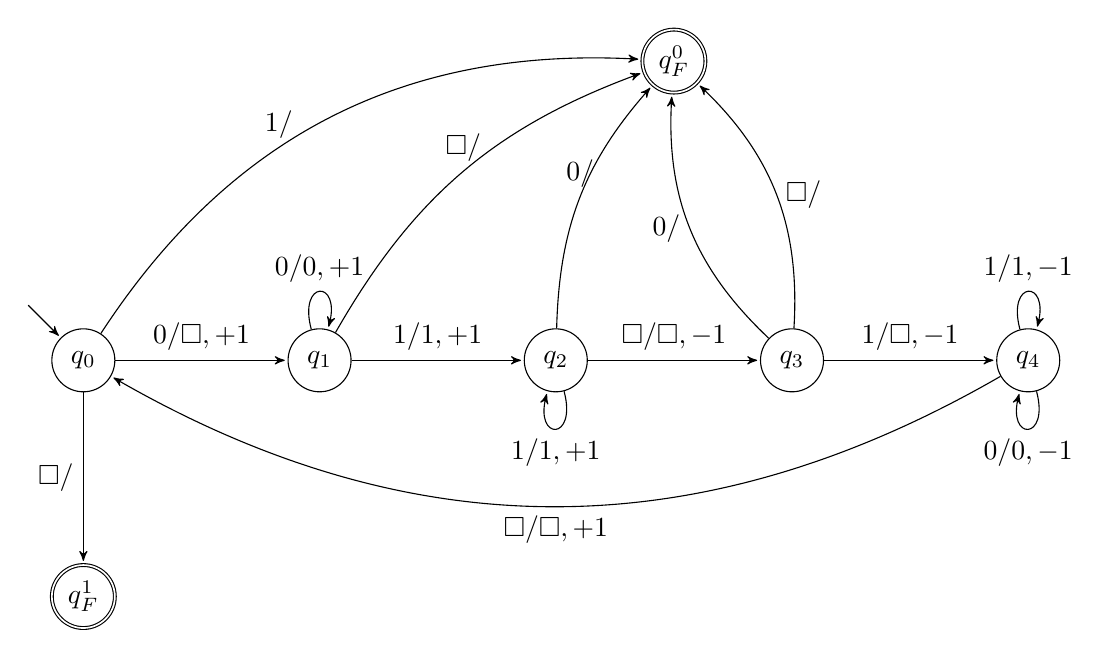
\begin{tikzpicture}[
    scale=1, transform shape,
    >=stealth', shorten >=1pt, auto,
    every state/.style={circle, draw, fill=white, minimum size=0.8cm, inner sep=1pt}
]
% Stati della riga principale
\node[state] (q0) at (0,0)    {$q_0$};
\node[state] (q1) at (3,0)    {$q_1$};
\node[state] (q2) at (6,0)    {$q_2$};
\node[state] (q3) at (9,0)    {$q_3$};
\node[state] (q4) at (12,0)   {$q_4$};

% Stati finali
\node[state, accepting] (qF0) at (7.5,3.8)  {$q_F^0$};
\node[state, accepting] (qF1) at (0,-3)     {$q_F^1$};

% Freccia d'ingresso
\draw[->] ([shift={(-0.7,0.7)}]q0.center) -- (q0);

% Transizioni lungo la riga principale
\draw[->] (q0) -- node {$0/\square,+1$} (q1);
\draw[->] (q1) -- node {$1/1,+1$} (q2);
\draw[->] (q2) -- node {$\square/\square,-1$} (q3);
\draw[->] (q3) -- node {$1/\square,-1$} (q4);

% Cappi
\draw[->] (q1) to[loop above, looseness=8] node {$0/0,+1$} (q1);
\draw[->] (q2) to[loop below, looseness=8] node {$1/1,+1$} (q2);
\draw[->] (q4) to[loop above, looseness=8] node {$1/1,-1$} (q4);
\draw[->] (q4) to[loop below, looseness=8] node {$0/0,-1$} (q4);

% Transizioni verso q_F^0 (rifiuto)
\draw[->] (q0) to[bend left=30]  node[pos=0.4, above] {$1/$}       (qF0);
\draw[->] (q1) to[bend left=20]  node[pos=0.5, above] {$\square/$} (qF0);
\draw[->] (q2) to[bend left=20]  node[pos=0.5, above] {$0/$}       (qF0);
\draw[->] (q3) to[bend left=25]  node[pos=0.5, left]  {$0/$}       (qF0);
\draw[->] (q3) to[bend right=25] node[pos=0.5, right] {$\square/$} (qF0);

% Transizione verso q_F^1 (accettazione)
\draw[->] (q0) -- node[swap] {$\square/$} (qF1);

% Ritorno da q_4 a q_0
\draw[->] (q4) to[bend left=30] node[pos=0.5, below] {$\square/\square,+1$} (q0);
\end{tikzpicture}
\caption{Macchina di Turing che decide $X=\{0^n1^n \mid n\geq 0\}$.}
\label{fig:turing-0n1n}
\end{figure}



\newpage

\section{Teoria della complessità}
\begin{defi}
    Data una macchina di Turing $\mu$ di alfabeto $A$ e insieme degli stati $Q$
    \[
    \mu: 
    Q\times  A' 
    \to Q' 
    \times 
    A' 
    \times 
    \{-1,+1\}
    \]
    con $A'=A \cup \{ \square\}$, $Q'=Q \cup \{ q_F^0, q_F^1\}$:
    \begin{enumerate}
        \item  sia
\[
C = (c_0,\dots,c_n)
\]
una computazione di $\mu$, il \textit{costo in tempo di $C$} è dato dalla lunghezza di $C$ diminuita di $1$;

\item il \textit{costo in spazio} è dato dalla cardinalità dell’insieme di interi $p$ tali che almeno per una delle configurazioni $c_i = (f_i,p_i,q_i)$ si ha $p= p_i$:
\[
|\{
p \, | \, (f,p,q) \in C
\}|;
\]

\item  si dirà che $\mu$ si arresta in tempo $t$ (rispettivamente spazio $s$) sull’input $w$, se $C$ è la computazione di
$\mu$ a partire dalla configurazione iniziale associata a $w$, $C$ raggiunge una configurazione terminale e il
costo in tempo di $C$ è $t$ ( rispettivamente il costo in spazio è $s$); in questo caso si userà la notazione
$T_\mu(w):A^* \to \mathbb N$ chiamata
\textit{funzione di tempo di arresto} 
(rispettivamente $S_\mu(w)$
$S_\mu(w):A^* \to \mathbb N$ chiamata
\textit{funzione di spazio di arresto} 
) per indicare il tempo di arresto $t$ (rispettivamente lo spazio di arresto
$s$).
    \end{enumerate}
\end{defi}
Di solito ci si interessa al comportamento nel caso peggiore:
\[
T_{max}(n)
:=
\operatorname{max}_{w\in A^*, \,|w|\leq n}T_\mu(w)
\]
Si noti che la definizione di costo in tempo di una computazione associata ad una parola da una macchina
di Turing si basa sulla lunghezza della computazione e pertanto si adatta a qualsiasi algoritmo formale (non
necessariamente per una macchina di Turing). Viceversa, per quanto riguarda la nozione di costo in spazio
la definizione è basata sulla specifica configurazione e pertanto non necessariamente è trasportabile nel caso
di altri algoritmi formali.
\begin{defi}
    Sia $\mu$ una macchina di Turing sull’alfabeto $A$ e con insieme di stati $Q$, e siano $T$, ed $S$ due
funzioni
$$T : \mathbb N \to \mathbb N,$$ $$S : \mathbb N \to \mathbb N.$$
Si dice che $\mu$ si \textit{arresta in tempo T} (rispettivamente \textit{in spazio S}) se per ogni $w\in A^*$ di lunghezza al più
uguale ad $n$ la macchina si arresta sull’input $w$ in tempo (risp. spazio) al più uguale a $T(n)$ (risp. $S(n)$).
\end{defi}
Infatti, quello che vorremmo è che
\[
T_\mu(w)\leq T(n), \quad \forall w \text{ tale che } {|w|\leq n}
\]
\begin{defi}

Siano $T$ e $S$ funzioni come nella definizione sopra.
\begin{enumerate}
    \item La macchina $\mu$ di alfabeto $A$ \emph{decide l'insieme $X$ in tempo $T$} (risp. \emph{spazio $S$}) se $\mu$ decide $X$ e se esiste un intero $N$ tale che per ogni intero $n \geq N$ e per ogni parola $w \in A^*$ di lunghezza al più uguale a $n$ la macchina $\mu$ si ferma a partire da $w$ in tempo al più uguale a $T(n)$ (risp. spazio al più uguale ad $S(n)$).

\item  La \textit{classe di complessità} $\mathrm{DTIME}_1^A(T)$ (risp. $\mathrm{DSPACE}_1^A(S)$) è l'insieme che contiene gli insiemi $X \subset A^*$ per i quali esiste almeno una macchina di Turing di alfabeto $A$ che decide $X$ in tempo $T$ (risp. in spazio $S$).
\end{enumerate}
\end{defi}
Con abuso di notazione, spesso scriveremo $T(n)$ invece che $T$.
\begin{rema}
    L'indice $1$ in basso utilizzato in questa notazione fa riferimento al fatto che nella macchina viene utilizzato un solo nastro.
 Con questa notazione si può notare che l'insieme $X$ degli interi divisibili per $9$ (come pure tutti gli insiemi decidibili per automa finito) appartengono alle classi $\mathrm{DTIME}_1^{\{0,1,\ldots,9\}}(n)$ e $\mathrm{DSPACE}_1^{\{0,1,\ldots,9\}}(n)$.
\end{rema}
È anche possibile interessarsi al caso medio, allora si prenderebbe in considerazione non la funzione $T_{max}$
ma una media su tutti i possibili input
\[
T_{avg} (n) :=
\frac{\sum_{w\in A^N}T_\mu(w)}{|A^N|}
\]
dove $A^N=\{ w\in A^* \,  |  \, |w| \leq N\}$.
\begin{defi}
 Una funzione
\[
T : \mathbb N \to \mathbb N
\]
viene detta \textit{funzione di complessità} se è una funzione non decrescente e se $T(n) \geq  n$ definitivamente.
\end{defi}
\subsection{Look-up Table}
Il lemma seguente mostra che il valore puntuale delle funzioni di complessità non corrisponde alla reale
difficoltà del problema, in quanto, data una macchina di Turing che decide un problema X con un certo
tempo di arresto, è sempre possibile trovarne un’altra che decide lo stesso problema con complessità lineare
per tutte le parole di input fino ad una lunghezza fissata, dunque la nozione di complessità ha senso come
misura della difficoltà di un problema solo quando si considera il comportamento asintotico dell’algoritmo.
\begin{lemm}[Look-up Table]
Dato un insieme $X \subset A^*$, supponiamo che esista una macchina di Turing $\mu$ che lo decide in tempo $T(n)$ e spazio $S(n)$.
Per un intero qualsiasi $N$ siano
\[
T'(n) =
\begin{cases}
n & n < N \\[4pt]
T(n) + 2N & \text{altrimenti}
\end{cases}
\]
e sia
\[
S'(n) =
\begin{cases}
n & n < N \\[4pt]
S(n) & \text{altrimenti}
\end{cases}
\]
allora esiste una macchina di Turing $\mu'$ che decide $X$ in tempo $T'(n)$ e spazio $S'(n)$.

\begin{proof}
Si può modificare la macchina $\mu$ per includere nell'insieme degli stati direttamente la risposta che corrisponde ad una data parola di input (in un numero finito di casi).

Ed è quello che faremo nel caso delle parole di lunghezza inferiore uguale ad $N$, in questo modo la nuova macchina si fermerà non appena sarà stata letta la parola di input. In questo caso la macchina dovrà leggere il nastro e quindi si arresterà in tempo al più $N$. In caso fossimo in presenza di una parola più lunga bisognerebbe riprendere la computazione della macchina $M$, reimpostando la macchina nello stato iniziale di $M$ e nella posizione iniziale.

Sia
\[
Q' = (Q\setminus \{ q_0\}) \cup \{q_w \mid w \in A^N\} \cup \{q_R, q_0^\mu\}
\]
dove lo stato $q_R$ sarà utilizzato come lo stato utilizzato per il ritorno alla casella iniziale nel caso in cui l'input si trovi più lungo di $N$ simboli.

Dunque la macchina di Turing $\mu'$ è definita a partire dalla macchina $\mu$:
\[
\mu'(q,a) =
\begin{cases}
\mu(a,q) & \text{se } q \in (Q\setminus\{q_0 \} )\cup \{q_0^\mu \}, \\[4pt]
(q_{wa}, a, +1) & \text{se } q = q_w \text{ per qualche } w \in A(m) \text{ con } m \le N \text{ e } |wa| \le N, \\[4pt]
(q_R, a, +1) & \text{se } q = q_w \text{ per qualche } w \in A(m) \text{ con } a \ne \square \text{ e } |w| = N, \\[4pt]
(q_R, a, -1) & \text{se } q = q_R \text{ e } a \ne \square, \\[4pt]
(q_0^\mu, a, +1) & \text{se } q = q_R \text{ e } a = \square, \\[4pt]
(q_F^1, a, +1) & \text{se } q = q_w \text{ per qualche } w \in A(m) \text{ con } m \le N,\ a = \square \text{ e } w \in X, \\[4pt]
(q_F^0, a, +1) & \text{se } q = q_w \text{ per qualche } w \in A(m) \text{ con } m \le N,\ a = \square \text{ e } w \notin X;
\end{cases}
\]
Lo stato iniziale $q_0'$ di $\mu'$ coincide con lo stato associato alla parola vuota $q_\epsilon$ mentre lo stato $q_0$ di $\mu$ viene pensato come lo stato aggiuntivo $q_0^\mu$.
Per ogni parola di lunghezza inferiore o uguale ad $N$ la computazione viene effettuata in modo simile alla computazione per automa finito, per le altre parole la macchina $\mu'$ compie una lettura ed un ritorno alla posizione iniziale che non altera l'input e dunque quando la macchina torna alla posizione iniziale e passa nello stato iniziale (di $\mu$) la computazione si svolge esattamente come per $\mu$.
\end{proof}
\end{lemm}
\textcolor{red}{Aggiugni grafico su dimostrazione.}
\begin{rema}
    Il nome "Look-up Table" nasce per il seguente motivo.
    La macchina che si costruisce 
    nella dimostrazione
    è la macchina di partenza ma che classifica
    già la decidibilità delle parole
    di lunghezza $N$.
    Poprio come se la macchina,
    alla prima lettura della parola, dovesse controllare in una "tavola"
    se la parola c'è (allora è accettata) o meno (allora viene scartata).
    Se la parola invece è più lunga di $N$,
    una volta che vengono letti 
    i primi
    $N$ caratteri,
    la macchina capisce che ci sono altri caratteri e allora,
    facendo altri $N$
    passi, torna all'inizio della parola e comincia ad analizzare la parola usando la strategia
    della macchina di Turing di partenza.
\end{rema}

\begin{rema} Il significato di questo lemma è che ha senso analizzare la complessità (dell'algoritmo di decisione associato), soltanto relativamente ad un insieme $X$ infinito, poiché nel caso di un $X$ finito si può sempre decidere il problema in un numero di passi finito, pari alla lunghezza della sua codifica sull'alfabeto (associando alla parola uno stato ``ad hoc'' e facendo una transizione accettante in base alla parola). Inoltre, poiché è possibile decidere il complementare di un insieme decidibile (invertendo nella tabella lo stato accettante $q_F^1$ e quello non accettante $q_F^0$), in pratica la questione della decidibilità si pone solo quando $X$ è infinito e co-infinito, mentre è banale quando l'insieme è finito oppure co-finito.
\end{rema}

\begin{rema} Il modello di calcolo ``macchina di Turing'' è più potente del modello ``automa a stati finiti'', in quanto per ogni automa $(T, q_0, F)$ resta definita una macchina di Turing $\mu$ sullo stesso alfabeto e sullo stesso insieme di stati per cui la computazione dell'algoritmo associato alla macchina $\mu$ coincide con l'algoritmo associato all'automa, più precisamente è sufficiente prendere
\[
\mu(q,a) :=
\begin{cases}
(T(q,a), a, +1) & a \ne \square \\[4pt]
(q_F^1, \square, +1) & \text{se } q \in F \\[4pt]
(q_F^0, \square, +1) & \text{se } q \notin F
\end{cases}
\]Ogni macchina di Turing associata ad un automa finito si arresta in tempo e spazio $T(n) = n$.    
\end{rema}
\begin{prop}
Sia $T : \mathbb{N} \to \mathbb{N}$ una funzione di complessità le inclusioni seguenti sono sempre vere.

\[
\mathrm{DTIME}_1^A(T) \subset \mathrm{DSPACE}_1^A(T) \subset \bigcup_{\epsilon > 0} \mathrm{DTIME}_1^A(2^{\epsilon T}).
\]

\begin{proof}

    Fissato l'alfabeto $A = \{0,1\}$, sia $X \in \mathrm{DTIME}_1^A(T)$. Poiché ad ogni passo di computazione è accessibile una sola posizione allora la massima posizione raggiungibile in $T(n)$ passi di computazione non può essere maggiore di $T(n)$.

Sia ora $\mu$ una macchina di Turing di alfabeto $A$ ed insieme degli stati $Q$, e sia $k = |A|$ e $d = |Q|$.

Per ogni intero $s$ esistono $(2s+1)k^{2s+1}d$ configurazioni distinte tali che coinvolgono durante la computazione soltanto le posizioni di indice compreso tra $1-s$ e $1+s$. Ora se il costo in spazio della computazione di $\mu$ a partire da una parola di input $w$ è maggiorato da $s$ (con $s$ più grande della lunghezza $|w|$) allora tutte le configurazioni coinvolgono posizioni di indice compreso tra $1-s$ e $1+s$. Quindi se la lunghezza della computazione fosse e solo se maggiore di $(2s+1)k^{2s+1}d$ si avrebbe necessariamente una configurazione ripetuta e perciò l'insieme delle configurazioni di $\mu$ a partire da $w$ sarebbe periodico, si avrebbe non terminazione, contraddicendo il fatto che nel caso peggiore la computazione termina in un tempo finito (dalla definizione di decidibilità). Quindi il tempo di arresto è certamente maggiorato da $(2s+1)k^{2s+1}d$ che per una costante $c$ abbastanza grande indipendente da $s$ si ha che il tempo di arresto è maggiorato da $2^{cs}$.
\end{proof}
\end{prop}



    


\newpage
\section{Prerequisiti}
Per tutto il documento, la definizione di funzione sarà quella di funzione parziale. Pertanto, data una funzione $f: A \to B$, indicheremo con $dom(f)$ il dominio della funzione $f$. Inoltre, se $x \in A \setminus dom(f)$ (quindi $f$ non è definita in $x$), allora scriveremo che $f(x):=\bot$.
Inoltre, qunado scriveremo \textit{alfabeto} intenderemo insieme.
Useremo la notazione $f^0:=\mathrm{Id}_x$ per ogni funzione $f:X \to X$. 
\begin{defi}[Funzione caratteristica]
La funzione $\mathbf{1}_X$ è la \textit{funzione caratteristica} (o indicatrice) dell'insieme $X$, definita come
\[
\mathbf{1}_X(w) = \begin{cases} 1 & w \in X \\ 0 & w \notin X. \end{cases}
\]
\end{defi}

\begin{defi}[Monoide]
    
\end{defi}

\begin{defi}[Partizione]
\end{defi}

\begin{defi}[Grafo etichettato]\label{def:grafo-etichettato}
Sia $A$ un insieme, detto \emph{alfabeto}. Un \emph{grafo etichettato} su $A$ è una terna
\[
G=(V,E,L),
\]
dove $E \subset V \times A \times V$ e
\begin{itemize}
    \item chiamando con $\pi_{1,3}$ la proiezione sulla prima e terza componente, $(V,\pi_{1,3}(E))$ è un grafo orientato;
    \item $L:E\to A$ è una funzione, detta \emph{funzione di etichettatura}, che associa ad ogni arco un elemento di $A$ chiamato \emph{etichetta} associata all'arco.
\end{itemize}
\end{defi}



\subsection{Semianelli e serie formali}
\label{sec:semianelli-serie-formali}

Per estendere ai grafi etichettati l'interpretazione combinatoria delle potenze successive della matrice di adiacenza, è necessario dotare l'insieme delle etichette di una struttura algebrica con somma e prodotto. Introduciamo qui, in modo autonomo, gli strumenti algebrici necessari: semianelli, matrici a coefficienti in un semianello, serie formali e algebre di Kleene.

\begin{defi}[Semigruppo]\label{def:semigruppo}
Un \emph{semigruppo} è una coppia $(S,\ast)$ dove $S$ è un insieme e
\[
\ast: S\times S \to S
\]
è un'operazione binaria (cioè una funzione che ad ogni coppia ordinata $(x,y)\in S\times S$ associa un elemento $x\ast y\in S$) tale che valga la proprietà associativa:
\[
(x\ast y)\ast z = x\ast(y\ast z) \qquad \text{per ogni } x,y,z\in S.
\]
\end{defi}

\begin{ex}
$(\mathbb{N},+)$ è un semigruppo: la somma di due numeri naturali è un numero naturale ed è associativa. Anche $(\mathbb{N},\cdot)$ è un semigruppo. Un altro esempio è $(A^*,\,\cdot\,)$, l'insieme delle stringhe finite su un alfabeto $A$ con l'operazione di concatenazione, che è associativa ma non commutativa se $|A|>1$.
\end{ex}

\begin{defi}[Semianello]\label{def:semianello}
Un \emph{semianello} è una struttura algebrica
\[
(S,+,\cdot)
\]
dove $S$ è un insieme e
\[
+: S\times S \to S, \qquad \cdot: S\times S \to S
\]
sono due operazioni binarie su $S$, dette rispettivamente \emph{somma} e \emph{prodotto}, tali che:
\begin{itemize}
    \item $(S,+)$ è un semigruppo (Definizione~\ref{def:semigruppo}), cioè $+$ è associativa;
    \item $(S,\cdot)$ è un semigruppo, cioè $\cdot$ è associativa;
    \item valgono le leggi di distribuzione tra somma e prodotto:
    \[
    x\cdot(y+z) = (x\cdot y) + (x\cdot z), \qquad (y+z)\cdot x = (y\cdot x) + (z\cdot x)
    \]
    per ogni $x,y,z\in S$.
\end{itemize}
\end{defi}

\begin{ex}
$(\mathbb{N},+,\cdot)$, con le usuali operazioni di somma e prodotto tra numeri naturali, è un semianello: non è un anello perché $(\mathbb{N},+)$ non ha elementi inversi (ad esempio non esiste $n\in\mathbb{N}$ tale che $2+n=0$).
Un secondo esempio, centrale per quanto segue, è il \emph{semianello booleano} $\mathbb{B}=(\{0,1\},\vee,\wedge)$, dove $\vee$ è l'operazione di ``or'' logico (che gioca il ruolo della somma modulo $2$) e $\wedge$ è l'operazione di ``and'' logico (che gioca il ruolo del prodotto modulo $2$).
\end{ex}

\begin{defi}[Semianello additivamente commutativo, zero, identità]\label{def:semianello-comm}
Sia $(S,+,\cdot)$ un semianello (Definizione~\ref{def:semianello}).
\begin{itemize}
    \item $(S,+,\cdot)$ si dice \emph{additivamente commutativo} se
    \[
    x+y=y+x \qquad \text{per ogni } x,y\in S.
    \]
    \item Un elemento $0\in S$ si dice \emph{zero} di $(S,+,\cdot)$ se
    \[
    x+0=0+x=x \quad \text{e} \quad x\cdot 0 = 0\cdot x = 0 \qquad \text{per ogni } x\in S.
    \]
    \item Un elemento $1\in S$ si dice \emph{identità} (o \emph{unità}) di $(S,+,\cdot)$ se
    \[
    x\cdot 1 = 1\cdot x = x \qquad \text{per ogni } x\in S.
    \]
\end{itemize}
Si noti che, quando esistono, lo zero e l'identità di un semianello sono unici: se $0$ e $0'$ fossero entrambi zeri, si avrebbe $0=0+0'=0'$; analogamente per l'identità.
\end{defi}

\begin{ex}
Nel semianello booleano $\mathbb{B}=(\{0,1\},\vee,\wedge)$ dell'esempio precedente, $0$ è lo zero (l'elemento neutro di $\vee$) e $1$ è l'identità (l'elemento neutro di $\wedge$): infatti $x\vee 0 = x$, $x\wedge 0 = 0$ e $x\wedge 1 = x$ per ogni $x\in\{0,1\}$. Il semianello $\mathbb{B}$ è inoltre additivamente commutativo, poiché $x\vee y = y\vee x$.
\end{ex}

\begin{defi}[Semianello idempotente]\label{def:semianello-idem}
Un semianello $(S,+,\cdot)$ additivamente commutativo, con zero $0$ e identità $1$ (Definizione~\ref{def:semianello-comm}), si dice \emph{idempotente} se l'operazione di somma è idempotente, ossia
\[
x+x=x \qquad \text{per ogni } x\in S.
\]
\end{defi}

\begin{ex}
Il semianello booleano $\mathbb{B}=(\{0,1\},\vee,\wedge)$ è idempotente: $x\vee x = x$ per ogni $x\in\{0,1\}$ (ad esempio $1\vee 1=1$). Al contrario, $(\mathbb{N},+,\cdot)$ non è idempotente, dato che ad esempio $1+1=2\neq 1$.
\end{ex}

\begin{defi}[Matrici su un semianello]\label{def:Mn}
Sia $S$ un insieme munito di struttura di semianello commutativo\footnote{Con \emph{commutativo}, quando non altrimenti specificato, si intende qui additivamente commutativo (Definizione~\ref{def:semianello-comm}).} con zero $0$ e identità $1$, e sia $n$ un intero positivo. Si definisce
\[
M_n(S) := \{ A : \{1,\dots,n\}\times\{1,\dots,n\} \to S \}
\]
l'insieme di tutte le matrici $n\times n$ a coefficienti in $S$ (cioè le funzioni che ad ogni coppia di indici $(i,j)$ associano un elemento $A_{ij}\in S$), munito delle operazioni:
\[
(A+B)_{ij} := A_{ij}+B_{ij} \qquad \text{(somma elemento per elemento)},
\]
\[
(A\cdot B)_{ij} := \sum_{k=1}^n A_{ik}\cdot B_{kj} \qquad \text{(prodotto righe per colonne)}.
\]
\end{defi}

Con tali operazioni $(M_n(S),+,\cdot)$ è a sua volta un semianello (le proprietà associative e distributive si verificano direttamente dalle corrispondenti proprietà in $S$), ed è in particolare un semigruppo additivamente commutativo se $S$ lo è. La matrice $0_n\in M_n(S)$ con tutti gli elementi uguali a $0$ è l'elemento neutro per l'operazione additiva, e la matrice identità
\[
I_n := \begin{pmatrix} 1 & 0 & \cdots & 0 \\ 0 & 1 & \cdots & 0 \\ \vdots & & \ddots & \vdots \\ 0 & 0 & \cdots & 1 \end{pmatrix} \in M_n(S)
\]
è l'identità del semianello $M_n(S)$.

Se $S$ contiene più di un elemento ed $n>1$, allora $M_n(S)$ non può essere moltiplicativamente commutativo (come nel caso classico delle matrici su un anello, è sufficiente esibire due matrici $A,B$ con $AB\neq BA$).

\begin{ex}
Per $n=2$ ed $S=\mathbb{B}$ il semianello booleano, si ha ad esempio
\[
A=\begin{pmatrix} 1 & 0 \\ 1 & 1\end{pmatrix}, \qquad B=\begin{pmatrix} 0 & 1 \\ 1 & 0\end{pmatrix} \quad \in M_2(\mathbb{B}),
\]
con prodotto (righe per colonne, usando $\vee,\wedge$ al posto di $+,\cdot$)
\[
A\cdot B = \begin{pmatrix} (1\wedge 0)\vee(0\wedge 1) & (1\wedge 1)\vee(0\wedge 0) \\ (1\wedge 0)\vee(1\wedge 1) & (1\wedge 1)\vee(1\wedge 0)\end{pmatrix} = \begin{pmatrix} 0 & 1 \\ 1 & 1\end{pmatrix}.
\]
\end{ex}

Per $A\in M_n(S)$ e $i,j\in\{1,\dots,n\}$, ricordiamo che $A_{ij}$ denota l'elemento di $A$ alla riga $i$-esima e alla colonna $j$-esima.

\begin{defi}[Trasposta]\label{def:trasposta}
La \emph{trasposta} di una matrice $A\in M_n(S)$ è la matrice $A^t\in M_n(S)$ definita da
\[
(A^t)_{ij} := A_{ji} \qquad \text{per ogni } i,j\in\{1,\dots,n\}.
\]
\end{defi}

Per ogni coppia di matrici $A,B\in M_n(S)$ valgono le identità
\[
(A^t)^t=A, \qquad (A+B)^t=A^t+B^t, \qquad (AB)^t=B^tA^t.
\]

\begin{ex}
Per la matrice $A$ dell'esempio precedente, $A^t = \begin{pmatrix} 1 & 1 \\ 0 & 1\end{pmatrix}$.
\end{ex}

\begin{defi}[Monoide]\label{def:monoide}
Un \emph{monoide} è una terna $(M,\cdot,1)$ dove $M$ è un insieme,
\[
\cdot: M\times M \to M
\]
è un'operazione binaria associativa (cioè $(M,\cdot)$ è un semigruppo, Definizione~\ref{def:semigruppo}), e $1\in M$ è un elemento tale che
\[
1\cdot m = m\cdot 1 = m \qquad \text{per ogni } m\in M.
\]
\end{defi}

\begin{ex}
Dato un alfabeto $A$, l'insieme $A^*$ delle stringhe finite su $A$ (incluso la stringa vuota $\epsilon$), munito dell'operazione di concatenazione e con elemento neutro $\epsilon$, è un monoide, detto \emph{monoide libero} generato da $A$.
\end{ex}

\begin{defi}[Serie formali]\label{def:serie-formali}
Dato un monoide $(M,\cdot,1)$ (Definizione~\ref{def:monoide}) e un semianello $\mathbb{K}$, si consideri l'insieme delle \emph{serie formali} a coefficienti in $\mathbb{K}$ sul monoide $M$:
\[
\mathbb{K}[M] := \left\{ \sum_{m\in M} \alpha_m\, m \;\middle|\; \alpha_m\in\mathbb{K} \text{ per ogni } m\in M \right\},
\]
cioè l'insieme delle funzioni $\alpha: M \to \mathbb{K}$, scritte formalmente come somme $\sum_{m\in M}\alpha_m m$ dove $\alpha_m:=\alpha(m)$.
\end{defi}

Su $\mathbb{K}[M]$ resta definita un'operazione di somma, elemento per elemento sui coefficienti,
\[
\sum_{m\in M}\alpha_m m \;+\; \sum_{m\in M}\beta_m m \;:=\; \sum_{m\in M}(\alpha_m+\beta_m)\, m,
\]
e un'operazione di prodotto (detta \emph{prodotto di convoluzione})
\[
\left(\sum_{m'\in M} \alpha_{m'}\, m'\right) \left(\sum_{m''\in M} \beta_{m''}\, m''\right) = \sum_{m\in M} \left( \sum_{\substack{m',m''\in M \\ m'm''=m}} \alpha_{m'}\beta_{m''} \right) m.
\]

Si noti che nella definizione di prodotto tra serie formali compaiono due nozioni distinte di prodotto:
\begin{itemize}
    \item il prodotto tra coefficienti $\alpha_{m'}\beta_{m''}$, che è il prodotto del semianello $\mathbb{K}$ (Definizione~\ref{def:semianello});
    \item il prodotto tra elementi del monoide $m'm''$, che è il prodotto del monoide $M$ (Definizione~\ref{def:monoide}).
\end{itemize}
Con queste due operazioni, $(\mathbb{K}[M],+,\cdot)$ è a sua volta un semianello.

\begin{ex}
Se $M=A^*$ è il monoide libero su un alfabeto $A$ e $\mathbb{K}=\mathbb{B}$ è il semianello booleano, una serie formale $\alpha\in\mathbb{B}[A^*]$ non è altro che un sottoinsieme $L\subseteq A^*$ (identificando $\alpha$ con la sua funzione caratteristica: $\alpha_m=1$ se $m\in L$, $\alpha_m=0$ altrimenti), cioè un \emph{linguaggio} su $A$. Il prodotto di convoluzione tra due serie $\alpha,\beta$ corrisponde in questo caso alla concatenazione di linguaggi
\[
L_1 \cdot L_2 = \{ w_1w_2 \mid w_1\in L_1,\, w_2\in L_2\}.
\]
\end{ex}

\begin{defi}[Ordine indotto da un semianello idempotente]\label{def:ordine}
Sia $(S,+,\cdot)$ un semianello idempotente (Definizione~\ref{def:semianello-idem}). Si definisce su $S$ la relazione binaria $\leq\,\subseteq S\times S$ data da
\[
a\leq b \quad\text{se e solo se}\quad a+b=b.
\]
\end{defi}

Si verifica facilmente che $\leq$ è un ordine parziale, ossia soddisfa:
\begin{itemize}
    \item \emph{riflessività}: $a\leq a$ per ogni $a\in S$ (segue da $a+a=a$, cioè dall'idempotenza);
    \item \emph{antisimmetria}: se $a\leq b$ e $b\leq a$ allora $a=b$ (da $a+b=b$ e $b+a=a$, usando la commutatività additiva, si ottiene $a=b+a=a+b=b$);
    \item \emph{transitività}: se $a\leq b$ e $b\leq c$ allora $a\leq c$ (da $a+b=b$ e $b+c=c$ segue $a+c = a+(b+c)=(a+b)+c=b+c=c$).
\end{itemize}

\begin{ex}
Nel semianello booleano $\mathbb{B}=(\{0,1\},\vee,\wedge)$, l'ordine indotto è quello usuale: $0\leq 1$, poiché $0\vee 1=1$.
\end{ex}

\begin{defi}[Estremo superiore]\label{def:sup}
Sia $(S,\leq)$ un insieme parzialmente ordinato (ad esempio quello indotto come in Definizione~\ref{def:ordine}) e sia $T\subseteq S$. Si dice che $y\in S$ è l'\emph{estremo superiore} di $T$, e si scrive $y=\sup T$, se e soltanto se:
\begin{enumerate}
    \item $x\leq y$ per ogni $x\in T$ (cioè $y$ è un maggiorante di $T$);
    \item per ogni $y'\in S$ che verifica la proprietà al punto (1), si ha $y\leq y'$ (cioè $y$ è il più piccolo dei maggioranti).
\end{enumerate}
\end{defi}

Per un insieme finito, l'estremo superiore è la somma degli elementi:
\[
\sup\{a_1,a_2\} = a_1+a_2, \qquad\qquad \sup\{a_1,\dots,a_n\} = a_1+\cdots+a_n.
\]
(Questo segue induttivamente dalla definizione di $\leq$: $a_1\leq a_1+a_2$ poiché $a_1+(a_1+a_2)=(a_1+a_1)+a_2=a_1+a_2$ per idempotenza, e analogamente per $a_2$; la minimalità segue dalla definizione di $+$ come somma nel semianello.)

Si noti che l'estremo superiore di un insieme infinito potrebbe non esistere in generale.

\begin{ex}
Nel semianello booleano, $\sup\{0,1\}=0\vee 1=1$, coerentemente con la formula generale.
\end{ex}

\begin{defi}[Algebra di Kleene]\label{def:kleene}
L'algebra delle serie formali $\mathbb{K}[M]$ (Definizione~\ref{def:serie-formali}) su un semianello idempotente $\mathbb{K}$ si dice \emph{algebra di Kleene} se ad ogni elemento $a\in\mathbb{K}$ è associato un elemento $a^*\in\mathbb{K}$, detto \emph{chiusura di Kleene} di $a$, tale che
\begin{equation}
a\, b^*\, c = \sup_{n\geq 0} a\, b^n\, c, \qquad \text{dove } b^n =
\begin{cases}
1 & \text{se } n=0 \\
b\cdot b^{n-1} & \text{se } n\geq 1,
\end{cases}
\label{eq:kleene-star}
\end{equation}
per ogni $a,b,c\in\mathbb{K}$, con il $\sup$ preso rispetto all'ordine parziale di Definizione~\ref{def:ordine}.
\end{defi}

L'equazione~\eqref{eq:kleene-star} asserisce, in particolare, la proprietà di chiusura mediante l'operatore $*$: postula l'esistenza dell'estremo superiore per famiglie infinite della forma $\{a\,b^n\,c\}_{n\geq0}$, anche quando l'esistenza del sup non è garantita in generale per un semianello idempotente qualsiasi.

\begin{ex}
Se consideriamo il semianello $\mathbb{B}[A^*]$ delle serie formali booleane sul monoide libero $A^*$ generato da un alfabeto $A$ (cioè, per l'esempio precedente, l'insieme dei linguaggi su $A$), si ottiene un'algebra di Kleene, [?, cap.~6, pag.~28], in cui la chiusura di Kleene di un linguaggio $L\subseteq A^*$ è data da
\[
L^* = \sum_{n\geq 0} L^n = \bigcup_{n\geq 0} L^n,
\]
cioè l'insieme di tutte le concatenazioni finite (incluso zero) di parole di $L$ — la classica operazione di chiusura di Kleene usata in teoria dei linguaggi formali.
\end{ex}

\newpage
\section{Wolfram}
\subsection{Introduzione}
\begin{rema}
Nel linguaggio Wolfram non ci sono tipi: l'unico tipo è il tipo \textit{funzione}.
Non c'è memoria, ma solo \textit{stati} (come per gli automi).
Si possono aggiungere stati e/o regole (queste ultime all'interno del ``kernel'' di Wolfram).
\end{rema}
\begin{defi}
Una \textit{espressione} è un oggetto della forma
\[
E[E_1, \dots, E_n]
\]
dove, a loro volta, gli $E_i$ sono espressioni.
\end{defi}
\begin{defi}
Data una funzione $f$ e un'espressione $E[E_1,\dots,E_n]$, si può costruire
\[
\wolfram{Map}[f, E[E_1, \dots, E_n]],
\]
che applica $f$ a ciascun argomento $E_i$, mantenendo la testa $E$.
\end{defi}
\begin{rema}
Ad esempio,
\[
\wolfram{Map}[f,\{a_1, \dots, a_n\}]
= \wolfram{Map}[f,\wolfram{List}[a_1, \dots, a_n]]
= \wolfram{List}[f[a_1], \dots, f[a_n]].
\]
\end{rema}
\begin{defi}
Ci sono due modi per introdurre regole nel kernel.
\begin{enumerate}
\item \textit{Assegnazione immediata} (\wolfram{=}): il membro destro viene \emph{valutato} e la regola di sostituzione così ottenuta viene inserita per tutte le espressioni che hanno la stessa forma:
\[
\wolfram{f[x_] = x + 2*a}
\]
\item \textit{Assegnazione ritardata} (\wolfram{:=}): il membro destro \emph{non} viene valutato, ma si memorizza soltanto la regola, che resta scritta così com'è:
\[
\wolfram{f[x_] := x + 2*a}
\]
\end{enumerate}
\end{defi}
\begin{rema}
Nel secondo caso la valutazione avviene solo quando si chiama, ad esempio, \wolfram{f[3]}: in quel momento vengono ricalcolate tutte le operazioni usando l'ultimo valore assegnato anche a tutti i parametri presenti nella regola.
\end{rema}
\begin{rema}
Esempio di codice:
\begin{walfram}
In[1]:=  f[x_] = 2x + a
Out[1]=  2x + a
In[2]:=  f[3]
Out[2]=  6 + a
In[3]:=  a = 2
Out[3]=  2
In[4]:=  f[3]
Out[4]=  8
\end{walfram}
Con \wolfram{=} il membro destro è stato valutato subito (con $a$ ancora indeterminato), mentre $a$ viene sostituito solo alla chiamata successiva.
\end{rema}
\begin{rema}
Per vedere le regole definite su un simbolo $f$ basta digitare
\[
\wolfram{?f}
\]
\end{rema}
\begin{defi}
Con \wolfram|List[1,2,3]| (o \wolfram|{1,2,3}|) si crea l'insieme ordinato $\{1,2,3\}$.
\end{defi}
\begin{defi}
Il comando
\[
\wolfram|Apply[k, {1,2,3}]|
\]
sostituisce la testa \wolfram{List} con $k$, dando come output
\[
k[1,2,3].
\]
\end{defi}
\begin{rema}
\wolfram{Plus} fa la somma degli elementi, quindi
\[
\wolfram|Apply[Plus, {1,2,3}]| \quad\longmapsto\quad 6.
\]
Cambiando \wolfram{Plus} in \wolfram{Times} si ottiene la produttoria:
\[
\wolfram|Apply[Times, {1,2,3}]| \quad\longmapsto\quad 6.
\]
\end{rema}
\begin{rema}
Per eseguire più istruzioni in un certo ordine, le si separa con un ``\wolfram{;}''. Il punto e virgola sopprime anche l'output dell'istruzione che precede.
\end{rema}
\begin{rema}
Esempio di codice:
\begin{walfram}
lista = Range[0, 1000]; Map[h, lista]
\end{walfram}
Il comando \wolfram{Range}
crea un'insieme
ordinato (in questo caso da $0$ a $1000$).
L'output è la lista $\{h[0], h[1], \dots, h[1000]\}$.
\end{rema}
\begin{defi}
Per estrarre elementi da una lista (o più in generale i rami dell'albero di un'espressione) si usa il comando \wolfram{Part}, comunemente abbreviato con le doppie parentesi quadre \wolfram{[[ ]]}. 
Ad esempio, se \wolfram{lista = \{a, b, c\}}, il comando \wolfram{lista[[2]]} restituisce \wolfram{b}. 
È possibile usarlo in modo annidato: \wolfram{matrice[[1, 2]]} estrae il secondo elemento della prima riga. In \wolfram{TM-lib.m}, \wolfram{automa[[1]]} estrae la tabella delle transizioni.
\end{defi}

\begin{defi}
In Wolfram è possibile definire \textit{funzioni pure} (o anonime) senza assegnare loro un nome. Si utilizza il simbolo \wolfram{\#} per indicare l'argomento (o gli argomenti, es. \wolfram{\#1, \#2}) e il simbolo \wolfram{\&} alla fine per indicare la chiusura della funzione. Ad esempio:
\[
\wolfram{Map[\#^2 \&, \{1, 2, 3\}]} \quad\longmapsto\quad \{1, 4, 9\}.
\]
Questo costrutto è estremamente comune per applicare trasformazioni rapide all'interno di un \wolfram{Map}.
\end{defi}

\begin{defi}
Oltre all'assegnazione globale 
(\wolfram{=}), esistono le \textit{regole di trasformazione} locali, create con \wolfram{->} (\wolfram{Rule}). Per applicare una o più regole a un'espressione si usa l'operatore di sostituzione \wolfram{/.} (\wolfram{ReplaceAll}). Ad esempio:
\[
\wolfram{x^2 + y  /.  x -> 3} \quad\longmapsto\quad 9 + y.
\]
Negli automi, le singole transizioni sono modellate proprio come liste di regole del tipo \wolfram{\{stato, simbolo\} -> nuovo\_stato}.
\end{defi}

\begin{rema}
Hai già visto che il comando \wolfram{Apply[f, espressione]} sostituisce la testa dell'espressione con \wolfram{f}. Esiste una forma sintattica abbreviata e molto diffusa per questa operazione, che usa il simbolo \wolfram{@@}. Pertanto:
\[
\wolfram{Apply[Plus, \{1, 2, 3\}]} \quad \text{è equivalente a} \quad \wolfram{Plus @@ \{1, 2, 3\}}.
\]
Nel codice della libreria, ad esempio, si usa \wolfram{Union @@ ...} per estrarre e unire in un unico insieme gli elementi di una lista di liste.
\end{rema}
\begin{defi}
In Wolfram Language, il costrutto \wolfram{Module} viene utilizzato per definire variabili locali. La sintassi generale è:
\[
\wolfram{Module[\{var1, var2, \dots\}, corpo\_della\_funzione]}
\]
Questo ambiente garantisce che le variabili dichiarate nella lista iniziale (ad esempio \wolfram{var1}, \wolfram{var2}) abbiano visibilità solo all'interno del modulo, evitando che vadano a sovrascrivere o interferire con variabili globali omonime definite altrove nel kernel.
\end{defi}

\begin{rema}
Il blocco \wolfram{Module} raggruppa più istruzioni separate da punto e virgola (\wolfram{;}) e restituisce come output il valore dell'ultima espressione valutata. Ad esempio:
\begin{walfram}
calcola[x_] := Module[{y, z},
  y = x^2;
  z = y + 1;
  z * 2
]
\end{walfram}
In questo caso, \wolfram{y} e \wolfram{z} sono variabili temporanee locali. L'output della chiamata \wolfram{calcola[3]} sarà il risultato dell'ultima operazione, ovvero \wolfram{20}.
\end{rema}
\subsection{Entropia}
\begin{defi}
Entropia \dots % da completare
\end{defi}
\begin{defi}
Sia $(\Omega,\mathcal{F},\mathbb{P})$ uno spazio di probabilità e sia $\mathcal{X}$ un insieme finito (l'alfabeto), munito della $\sigma$-algebra $2^{\mathcal{X}}$. Una variabile aleatoria è una funzione misurabile $X\colon \Omega \to \mathcal{X}$. La sua legge è la misura di probabilità $\mathbb{P}_X = \mathbb{P}\circ X^{-1}$ su $\mathcal{X}$, e si pone
\[
p(x) = \mathbb{P}_X(\{x\}) = \mathbb{P}(X = x), \qquad x \in \mathcal{X}.
\]
\end{defi}
\begin{defi}
Il \textit{contenuto informativo} (grezzo) di un esito $x\in\mathcal{X}$ con $p(x)>0$ è
\[
h(x) = \log \frac{1}{p(x)} = -\log p(x).
\]
Con il logaritmo in base $2$ l'unità di misura è il bit. Più un esito è improbabile, maggiore è la sua informazione: $h(x)=0$ se e solo se $p(x)=1$.
\end{defi}
\begin{defi}
Date due variabili aleatorie $X\colon\Omega\to\mathcal{X}$ e $Y\colon\Omega\to\mathcal{Y}$, la loro legge congiunta è $p(x,y)=\mathbb{P}(X=x,\,Y=y)$. Il contenuto informativo della coppia è
\[
h(x,y) = \log \frac{1}{p(x,y)}.
\]
\end{defi}
\begin{defi}
Le variabili $X$ e $Y$ sono \textit{indipendenti} se $\sigma(X)$ e $\sigma(Y)$ sono indipendenti, cioè $\mathbb{P}(X\in A,\, Y\in B)=\mathbb{P}(X\in A)\,\mathbb{P}(Y\in B)$ per ogni $A\subseteq\mathcal{X}$ e $B\subseteq\mathcal{Y}$. Poiché gli alfabeti sono finiti, ciò equivale a
\[
p(x,y) = p(x)\,p(y) \qquad \forall\, x\in\mathcal{X},\ y\in\mathcal{Y}.
\]
\end{defi}
\begin{rema}
Se $X$ e $Y$ sono indipendenti, allora l'informazione della coppia è la somma delle informazioni:
\[
h(x,y) = \log\frac{1}{p(x)\,p(y)} = \log\frac{1}{p(x)} + \log\frac{1}{p(y)} = h(x) + h(y).
\]
Questa è la ragione per cui si usa il logaritmo: trasforma il prodotto delle probabilità (indipendenza) in una somma di informazioni.
\end{rema}
\begin{defi}
L'\textit{entropia} di $X$ è il valore atteso del contenuto informativo:
\[
H(X) = \mathbb{E}\big[h(X)\big] = \int_{\Omega} h\big(X(\omega)\big)\, d\mathbb{P}(\omega).
\]
Per il teorema di cambio di variabili rispetto alla legge $\mathbb{P}_X$ si ottiene
\[
H(X) = \int_{\mathcal{X}} h(x)\, d\mathbb{P}_X(x) = \sum_{x\in\mathcal{X}} p(x)\, h(x) = \sum_{x\in\mathcal{X}} p(x)\log\frac{1}{p(x)},
\]
con la convenzione $0\log\frac{1}{0}=0$, che permette di sommare anche sugli $x$ con $p(x)=0$.
\end{defi}
\begin{rema}
L'entropia misura l'informazione media, o equivalentemente l'incertezza, associata a $X$. Dipende solo dalla legge $\mathbb{P}_X$ e non dai valori assunti da $X$. Vale sempre $H(X)\ge 0$, poiché $h(x)\ge 0$ quando $p(x)>0$. Inoltre, essendo $\mathcal{X}$ finito, $h(X)$ è una funzione semplice e quindi integrabile, dunque $H(X)<\infty$.
\end{rema}
\begin{rema}
Se $X$ e $Y$ sono indipendenti, $H(X,Y)=H(X)+H(Y)$. Infatti, per la linearità del valore atteso e l'additività di $h$,
\[
H(X,Y) = \mathbb{E}\big[h(X,Y)\big] = \mathbb{E}\big[h(X)+h(Y)\big] = \mathbb{E}\big[h(X)\big] + \mathbb{E}\big[h(Y)\big] = H(X) + H(Y).
\]
\end{rema}
\begin{rema}
Esempio di calcolo dell'entropia (in bit) di una distribuzione $p=(\tfrac12,\tfrac14,\tfrac14)$:
\begin{walfram}
p = {1/2, 1/4, 1/4};
Total[p * Log[2, 1/p]]
\end{walfram}
L'output è $\tfrac{3}{2}$, infatti $\tfrac12\cdot 1+\tfrac14\cdot 2+\tfrac14\cdot 2=\tfrac32$.
\end{rema}
\begin{defi}
Appendice: fondamenti di probabilità. Uno \textit{spazio di probabilità} è una terna $(\Omega,\mathcal{F},\mathbb{P})$ dove:
\begin{itemize}
\item $\mathcal{F}\subseteq 2^{\Omega}$ è una $\sigma$-algebra, cioè $\Omega\in\mathcal{F}$, è chiusa per complementare e per unioni numerabili;
\item $\mathbb{P}\colon\mathcal{F}\to[0,1]$ è una misura con $\mathbb{P}(\Omega)=1$, cioè è $\sigma$-additiva sugli elementi disgiunti di $\mathcal{F}$.
\end{itemize}
Una funzione $X\colon(\Omega,\mathcal{F})\to(E,\mathcal{E})$ è \textit{misurabile} se $X^{-1}(A)\in\mathcal{F}$ per ogni $A\in\mathcal{E}$. La \textit{legge} di $X$ è $\mathbb{P}_X(A)=\mathbb{P}(X^{-1}(A))$ per $A\in\mathcal{E}$.
\end{defi}
\begin{defi}
Sia $g\colon\Omega\to\mathbb{R}$ misurabile. Il \textit{valore atteso} di $g$ è l'integrale di Lebesgue
\[
\mathbb{E}[g] = \int_{\Omega} g\, d\mathbb{P},
\]
definito prima per le funzioni semplici $g=\sum_{i} c_i \mathbbm{1}_{A_i}$ come $\sum_i c_i\,\mathbb{P}(A_i)$, poi per $g\ge0$ come estremo superiore sulle funzioni semplici $0\le s\le g$, e infine per $g$ integrabile come $\mathbb{E}[g^+]-\mathbb{E}[g^-]$.
\end{defi}
\begin{rema}
Vale il \textit{cambio di variabili}: se $X\colon\Omega\to E$ è misurabile e $f\colon E\to\mathbb{R}$ è misurabile e integrabile rispetto a $\mathbb{P}_X$, allora
\[
\mathbb{E}\big[f(X)\big] = \int_{\Omega} f\circ X\, d\mathbb{P} = \int_{E} f\, d\mathbb{P}_X.
\]
Se $E$ è finito o numerabile, l'ultimo integrale si riduce alla somma $\sum_{x\in E} f(x)\,\mathbb{P}_X(\{x\})$. Questa è la formula usata per scrivere $H(X)=\sum_x p(x)h(x)$.
\end{rema}
\begin{rema}
Calcoliamo \wolfram|Integrate[x^2 Sin[x], x]| e vediamo il risultato:
\[
\int x^2 \sin x \, dx = (2 - x^2)\cos x + 2x \sin x + C.
\]
\end{rema}
\subsection{Libreria TM-lib}
\begin{defi}
Per implementare gli automi in Wolfram si usa il pacchetto \wolfram{TM-lib.ma}. Si procede in tre passi.
\begin{enumerate}
\item Assegnare la directory corrente, cioè la cartella che contiene il pacchetto: \wolfram|SetDirectory["/percorso/della/cartella"]|
\item Caricare la libreria: \wolfram|Get["TM-lib.ma"]|
\item Usare le funzioni implementate dalla libreria (elencate sotto).
\end{enumerate}
\end{defi}
\begin{rema}
Esempio di codice per i primi due passi:
\begin{walfram}
SetDirectory["/percorso/della/cartella"]
Get["TM-lib.ma"]
\end{walfram}
\end{rema}
\begin{defi}
La libreria implementa le seguenti funzioni.
\begin{itemize}
\item \wolfram|ShowConfiguration[c_]| visualizza la configurazione (di una macchina di Turing).
\item \wolfram|ManipulateComputation[mu_, init_]| visualizza la computazione di una macchina di Turing.
\item \wolfram|InitAutomaton[automaton_, w_]| inizializza l'automa, cioè restituisce la configurazione iniziale associata alla parola $w$.
\item \wolfram|DFA2TM[automaton_]| trasforma un automa nella macchina di Turing equivalente.
\item \wolfram|States[automaton_]| restituisce la lista degli stati dell'automa.
\item \wolfram|ProductFinalStates[A1_, A2_]| restituisce l'automa prodotto a partire da due automi (composizione parallela).
\item \wolfram|TuringMachineGraph[mu_]| restituisce il grafo della macchina di Turing.
\end{itemize}
\end{defi}
\begin{rema}
Nelle firme delle funzioni il carattere \wolfram{_} indica un \emph{pattern}, cioè un parametro formale. Quando si chiama la funzione si scrive solo l'argomento, senza il trattino basso.
\end{rema}
\subsection{Automi}
\begin{defi}
Un automa si specifica con tre oggetti:
\begin{itemize}
\item la lista \wolfram{T} delle transizioni, ciascuna della forma \wolfram|{stato, simbolo} -> nuovo_stato|;
\item lo stato iniziale \wolfram{q0};
\item l'insieme \wolfram{F} degli stati finali.
\end{itemize}
L'automa è la terna \wolfram|{T, q0, F}|.
\end{defi}
\begin{rema}
Esempio di automa con due stati, \wolfram{pari} e \wolfram{dispari}, sull'alfabeto $\{0,1\}$. Lo stato cambia a ogni simbolo $1$ letto e resta invariato a ogni simbolo $0$, quindi l'automa accetta le parole con un numero pari di $1$.
\begin{walfram}
T = {
  {pari, 0} -> pari,
  {dispari, 0} -> dispari,
  {pari, 1} -> dispari,
  {dispari, 1} -> pari
  }
q0 = pari
F = {pari}
automa = {T, q0, F}
\end{walfram}
Per mostrare l'esecuzione:
\begin{walfram}
init = InitAutomaton[
    automa2, {0, 1, 1, 0, 0, 1, 1, 1, 1, 1, 0, 0, 0, 1}
    ] ;
mu = DFA2TM[automa2] ;
TuringMachineGraph[mu]
ManipulateComputation[mu, init]
\end{walfram}
\end{rema}
\begin{rema}
Una volta definito \wolfram{automa}, lo si può inizializzare su una parola $w$ con \wolfram|InitAutomaton[automa, w]|, che restituisce la configurazione iniziale. Con \wolfram|DFA2TM[automa]| si ottiene la macchina di Turing equivalente, di cui si può visualizzare la computazione con \wolfram|ManipulateComputation| e il grafo con \wolfram|TuringMachineGraph|.
\end{rema}
\begin{rema}
\textbf{Composizione di automi:}
Per studiare sistemi complessi o l'intersezione di linguaggi regolari, la libreria mette a disposizione il prodotto cartesiano tramite le funzioni \wolfram{ProductTable[A1, A2]} e \wolfram{ProductFinalStates[A1, A2]}. 
La prima genera le transizioni incrociate combinando gli stati con il comando \wolfram{Tuples}, mentre la seconda definisce gli stati finali dell'automa prodotto.
\end{rema}

\begin{defi}
La funzione di visualizzazione interattiva
\[
\wolfram{ManipulateComputation[mu, init]}
\]
combina il motore di animazione di Wolfram (\wolfram{Manipulate}) con la generazione sequenziale delle configurazioni della macchina di Turing, permettendo di scorrere passo-passo l'intera computazione fino al limite di passi predefinito (\wolfram{maxsteps}).
\end{defi}

\newpage
\section{Esercizi}
\subsection{Automi}
\begin{ex}\label{es:1}
Fissiamo l'alfabeto binario $A=\{0,1\}$, dimostrare che l'insieme
\[
X = \{ w0 \mid w\in A^* \}
\]
è decidibile per automa a stati finiti.


\begin{sol} Si richiede di mostrare un automa il cui algoritmo associato accetta le parole che terminano con uno zero. È dunque sufficiente memorizzare nello stato l'ultimo simbolo letto e alla fine della lettura della parola decidere in base allo stato: poniamo $Q=\{q_0,q_1\}$, e definiamo
\[
T(q,a) :=
\begin{cases}
q_0 & \text{se } a=0, \\
q_1 & \text{se } a=1,
\end{cases}
\]
prendiamo $q_0$ come stato iniziale e $F=\{q_0\}$ come insieme degli stati finali accettanti.
.
Sia
\[
X=\{w0\mid w\in A^*\}
\]
l'insieme delle parole sull'alfabeto binario che terminano con il simbolo \(0\).

Costruiamo un automa finito che decide \(X\). Consideriamo l'insieme degli stati
\[
Q=\{q_0,q_1\},
\]
dove intuitivamente:
\begin{itemize}
    \item \(q_0\) rappresenta la situazione in cui l'ultimo simbolo letto è \(0\);
    \item \(q_1\) rappresenta la situazione in cui l'ultimo simbolo letto è \(1\).
\end{itemize}

Definiamo la funzione di transizione
\[
T:Q\times A\to Q
\]
come
\[
T(q,a)=
\begin{cases}
q_0 & \text{se } a=0,\\
q_1 & \text{se } a=1.
\end{cases}
\]

Scegliamo come stato iniziale
\[
q_{\mathrm{init}}=q_0
\]
e come insieme degli stati accettanti
\[
F=\{q_0\}.
\]

Consideriamo ora l'algoritmo associato all'automa.
Sia
\[
w=a_1a_2\cdots a_n\in A^*.
\]
La configurazione iniziale è
\[
\epsilon(w)=(w,1,q_0).
\]

Dopo \(k\) transizioni, per induzione su \(k\), la configurazione raggiunta è
\[
(w,k+1,q_k),
\]
dove
\[
q_k=
\begin{cases}
q_0 & \text{se } a_k=0,\\
q_1 & \text{se } a_k=1.
\end{cases}
\]

Infatti, ad ogni passo la funzione di transizione sostituisce lo stato corrente con lo stato corrispondente all'ultimo carattere letto.

Dopo aver letto tutta la parola \(w\), la computazione termina nella configurazione
\[
(w,n+1,q_n).
\]
La funzione di uscita restituisce quindi
\[
\delta(w,n+1,q_n)=
\begin{cases}
1 & \text{se } q_n\in F,\\
0 & \text{se } q_n\notin F.
\end{cases}
\]

Poiché
\[
F=\{q_0\},
\]
si ha
\[
\delta(w,n+1,q_n)=
\begin{cases}
1 & \text{se l'ultimo simbolo di } w \text{ è }0,\\
0 & \text{se l'ultimo simbolo di } w \text{ è }1.
\end{cases}
\]

Quindi
\[
f_{\mathcal A}(w)=
\begin{cases}
1 & \text{se } w\in X,\\
0 & \text{se } w\notin X.
\end{cases}
\]

Pertanto
\[
f_{\mathcal A}=\mathbf 1_X
\]
e quindi l'algoritmo associato all'automa decide \(X\).

Concludiamo che
\[
X=\{w0\mid w\in A^*\}
\]
è DFA-decidibile.
\end{sol}
\end{ex}

\newpage

\begin{ex}\label{es:3}
Si consideri l'alfabeto $A=\{0,1\}$ e sia $B=\{1\}$ la restrizione all'insieme che contiene il solo simbolo $1$; si considerino l'insieme delle parole di alfabeto $A$ di lunghezza pari:
\[
X_1 = \{ w \in A^* \mid |w| = 2n,\ n\geq 0 \}
\]
e l'insieme delle parole di alfabeto $A$ che contengono un numero pari di $1$:
\[
X_2 = \{ w \in A^* \mid |w_{|B}| = 2k,\ k\geq 0 \}
\]
qui si è utilizzata la notazione $w_{|B}$ per indicare la parola $w$ 
ristretta ai soli elementi di alfabeto $B$.
Costruire l'automa che decide $X_1+X_2$.

\begin{sol}
Utilizzando il teorema 
\ref{prop:8},
basta esibire gli automi che decidono $X_1$ e $X_2$.
L'automa che decide $X_1$ è quello dell'esempio 
\ref{ex: parole lunghezze pari} (il grafo corrsipondente e' nella figura 
\ref{figura esempio automa per parole pari}).
Definiamo ora l'automa che decide $X_2$.
Definiamo $Q_2=\{q_0, q_1 \}$ dove $q_0$ e/' sia stato iniziale che stato accettante, mentre $q_1$ e/' uno stato non accettante.
E definiamo la funzione di transizione $T_2$ come segue:
\[
\begin{matrix}  
T_2: & Q_2 \times A & \to  & Q_2
\\
& (q_0,0) & \mapsto & q_0\\
& (q_0,1) & \mapsto & q_1\\
& (q_1,0) & \mapsto & q_1\\
& (q_1,1) & \mapsto & q_0   
\end{matrix}
\]
In questo modo, l'automa che decide $X_2$ 
accetta le parole che contengono un numero pari di $1$
(si guardi il grafico dell'automa nella figura \ref{fig:parita}).
A questo punto,
utilizzando la costruzione 
effettuata
nella dimostrazione 
del teorema \ref{prop:8}
otteniamo che l'automache decide 
$X_1 + X_2$
e/' l'automa
\[
\begin{cases}
    Q:= Q_1 \times Q_2,\\
    q_0 := (q_0',q_0''),\\
    F := (F_1 \times Q_2) \cup (Q_1 \times F_2),\\
    T((q_1,q_2),a) = (T_1(q_1,a), T_2(q_2,a))
\end{cases}
\]
dove con un apice indichiamo gli stati di dell'automa che decide 
$X_1$ e con due apici gli stati dell'automa che decide $X_2$.
Per completezza,
presentiamo il grafo dell'automa che decide $X_1 + X_2$
(che puo/' esssere disegnato a partire dall'automa appena definito
oppure usando i grafi degli automi che decidono $X_1$ e $X_2$).
\begin{center}
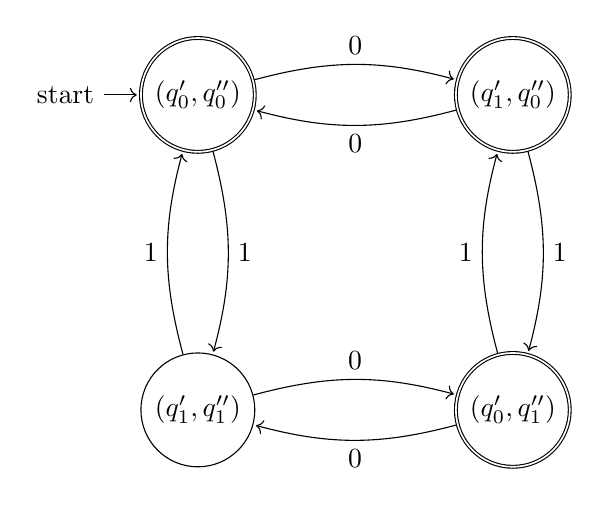
\begin{tikzpicture}[shorten >=1pt, node distance=4cm, on grid, auto]
   % Stati disposti a quadrato seguendo il ciclo delle transizioni
   \node[state, initial, accepting] (q00) {$(q_0', q_0'')$};
   \node[state, accepting]          (q10) [right=of q00] {$(q_1', q_0'')$};
   \node[state, accepting]          (q01) [below=of q10] {$(q_0', q_1'')$};
   \node[state]                     (q11) [left=of q01]  {$(q_1', q_1'')$};

   % Transizioni senza intersezioni
   \path[->]
    % Bordo superiore (Transizioni con 0)
    (q00) edge [bend left=15] node {0} (q10)
    (q10) edge [bend left=15] node {0} (q00)
    
    % Bordo destro (Transizioni con 1)
    (q10) edge [bend left=15] node {1} (q01)
    (q01) edge [bend left=15] node {1} (q10)
    
    % Bordo inferiore (Transizioni con 0)
    (q01) edge [bend left=15] node {0} (q11)
    (q11) edge [bend left=15] node {0} (q01)
    
    % Bordo sinistro (Transizioni con 1)
    (q11) edge [bend left=15] node {1} (q00)
    (q00) edge [bend left=15] node {1} (q11);
\end{tikzpicture}
\end{center}
\end{sol}
\end{ex}

\end{document}
